% \documentclass[a4paper,10pt]{article}
\documentclass[review]{siamart}
\usepackage{url}
\usepackage{amssymb}
\usepackage{amsmath}
\usepackage{bm}
\usepackage{stmaryrd}
\usepackage{array}
\usepackage{multirow}
\usepackage{empheq}
\usepackage{enumitem}
	\setlist{nosep} % or \setlist{noitemsep} to leave space around whole list
\usepackage{color}
\usepackage{verbatim}
\usepackage{showlabels}
\usepackage{adjustbox}
\usepackage{hyperref}
\definecolor{darkgreen}{rgb}{0.0, 0.5, 0}
\usepackage[numbers,sort]{natbib}
\usepackage{cleveref}
\usepackage[belowskip=-5pt]{subcaption}

\newsiamremark{remark}{Remark}
\newsiamremark{assumption}{Assumption}


% \newtheorem{lemma}{Lemma}
% \newtheorem{definition}{Definition}
% \newtheorem{theorem}{Theorem}
% \newtheorem{corollary}{Corollary}

\newcommand{\tcb}{\textcolor{blue}}
\newcommand{\tcp}{\textcolor{purple}}
\newcommand{\todo}[1]{\textcolor{red}{[TODO\@: #1]}}

\newcommand{\mdet}{\operatorname{det}}
\newcommand{\madj}{\operatorname{adj}}

% ------------------------------------------------------------------------------------ %
% ------------------------------------------------------------------------------------ %

\newcommand{\TheTitle}{Fast parallel solution of fully implict Runge-Kutta and discontinous
	Galerkin in time for numerical PDEs, Part II: the nonlinear setting}
\newcommand{\TheAuthors}{B.S. Southworth, O. Krzysik, and W. Pazner}
\headers{Parallel solution of fully implict Runge-Kutta and DG in time I}{\TheAuthors}
\title{{\TheTitle}\thanks{This research was conducted ...
  }}

\author{Ben S. Southworth\thanks{Department of Applied Mathematics,
    University of Colorado,
    U.S.A. (\url{ben.s.southworth@gmail.com}),
    \url{http://orcid.org/0000-0002-0283-4928}}
    \and
    Oliver Krzysik
  	\thanks{School of Mathematical Sciences, Monash University,
  	Australia (\url{oliver.krzysik@monash.edu})}
  	\and
  	Will Pazner\thanks{Lawrence Livermore National Laboratory,
    U.S.A. (\url{pazner1@llnl.gov})}
}

\ifpdf%
\hypersetup{%
  pdftitle={\TheTitle},
  pdfauthor={\TheAuthors}
}
\fi

% ------------------------------------------------------------------------------------ %
% ------------------------------------------------------------------------------------ %

\begin{document}
\maketitle
\allowdisplaybreaks

\begin{abstract}

\end{abstract}


% ------------------------------------------------------------------------------------- %
% ------------------------------------------------------------------------------------- %
% ------------------------------------------------------------------------------------- %
\section{Introduction}\label{sec:intro}

% ------------------------------------------------------------------------------------- %
% ------------------------------------------------------------------------------------- %
\subsection{Fully implicit Runge-Kutta}\label{sec:intro:irk}

Consider the method-of-lines approach to the numerical solution of partial differential
equations (PDEs), where we discretize in space and arrive at a system of ordinary
differential equations (ODEs) in time,
%
\begin{align}\label{eq:problem}
	M\mathbf{u}'(t) =  \mathcal{N}(\mathbf{u},t) \quad\text{in }(0,T], \quad \mathbf{u}(0) = \mathbf{u}_0,
\end{align}
%
where $M$ is a mass matrix and $\mathcal{N}\in\mathbb{R}^{N\times N}$ is a discrete, time-dependent, nonlinear operator depending on $t$ and $\mathbf{u}$ (including potential
forcing terms).\footnote{Note, PDEs with an algebraic constraint, for example, the divergence-free
constraint in Navier Stokes, instead yield a differential algebraic equation (DAE), which
requires separate careful treatment and will be the subject of a forthcoming paper.}
Then, consider time propagation using an $s$-stage Runge-Kutta scheme,
characterized by the Butcher tableaux 
%
\begin{align*}
	\renewcommand\arraystretch{1.2}
	\begin{array}
	{c|c}
	\mathbf{c}_0 & A_0\\
	\hline
	& \mathbf{b}_0^T
	\end{array},
\end{align*}
%
with Runge-Kutta matrix $A_0 = (a_{ij})$, weight vector $\mathbf{b}_0^T = (b_1, \ldots, b_s)^T$,
and quadrature nodes $\mathbf{c}_0 = (c_0, \ldots, c_s)$.

Runge-Kutta methods update the solution using a sum over stage vectors,
%
\begin{align}\label{eq:update}
\mathbf{u}_{n+1} & = \mathbf{u}_n + \delta t \sum_{i=1}^s b_i\mathbf{k}_i, \\
M\mathbf{k}_i & = \mathcal{N}\left(\mathbf{u}_n + \delta t\sum_{j=1}^s a_{ij}\mathbf{k}_j, t_n+\delta tc_i\right).\label{eq:stages}
\end{align}
%
For nonlinear PDEs, $\mathcal{N}$ is linearized using, for example, a Newton or a Picard
linearization of the underlying PDE. Let us denote this linearization
${\mathcal{L}}\in\mathbb{R}^{N\times N}$
(or, in the case of a linear PDE, let $\mathcal{L} := \mathcal{N}$).
Expanding, solving for the stages $\mathbf{k}$ as each step in a nonlinear iteration, or
as the update to $\mathbf{u}$ for a linear PDE, can then be expressed as the
solution of the block linear system,
%
\begin{align}\label{eq:k0}
\left( \begin{bmatrix} M  & & \mathbf{0} \\ & \ddots \\ \mathbf{0} & & M\end{bmatrix}
	- \delta t \begin{bmatrix} a_{11}\mathcal{L}_1 & ... & a_{1s}\mathcal{L}_1 \\
	\vdots & \ddots & \vdots \\ a_{s1}\mathcal{L}_s & ... & a_{ss} \mathcal{L}_s \end{bmatrix} \right)
	\begin{bmatrix} \mathbf{k}_1 \\ \vdots \\ \mathbf{k}_s \end{bmatrix} 
& = \begin{bmatrix} \mathbf{f}_1 \\ \vdots \\ \mathbf{f}_s \end{bmatrix}.
\end{align}
%

The difficulty in fully implicit Runge-Kutta methods (which we will denote IRK) lies in
solving the $Ns\times Ns$ block linear system in \eqref{eq:k0}. This paper focuses on the
parallel simulation of numerical PDEs, where $N$ is typically very large
and $\mathcal{L}$ is highly ill-conditioned. In such cases, direct
solution techniques to solve \eqref{eq:k0} are not a viable option, and fast, parallel 
iterative methods must be used. However, IRK methods are rarely employed in practice due
to the difficulties of solving \eqref{eq:k0}. Even for relatively simple
parabolic PDEs where $\mathcal{L}$ is symmetric positive definite, \eqref{eq:k0}
instead yields a large nonsymmetric system with significant block coupling. For
nonsymmetric systems $\mathcal{L}$ that already have variable coupling, fast iterative
methods are even less likely to yield acceptable performance in solving \eqref{eq:k0}.

% ------------------------------------------------------------------------------------- %
% ------------------------------------------------------------------------------------- %
\subsection{Discontinuous Galerkin in time}\label{sec:intro:dg}

Another field that has seen growing interest recently for numerical PDEs is discretizing
in time using finite elements, rather than standard ODE techniques. Some of the more
interesting features of using finite-elements in time is the natural ability to handle
time-dependent domains, unstructured meshes in space-time, and adaptive mesh
refinement in space and time. However, for so-called slab-based meshing in time with
discontinuous Galerkin finite elements, where
the time domain is discretized using spatial slabs (that is, the same time step is
applied to the entire spatial domain), the resulting linear systems that must be
solved for each time step take the same structure as \eqref{eq:k0} (for example,
see \cite{hn}). A handful of works have looked at linear solvers for such
discretizations, primarily for parabolic problems, including block preconditioning
approaches \cite{exh,8jp,27n}, and direct space-time multigrid methods 
\cite{gander2016analysis}.

Although this paper focuses on fully implicit Runge-Kutta, the algorithms developed
here can be directly applied to discontinuous Galerkin discretizations in time on
fixed slab-based meshes. In fact, the principles used in this paper are similar
to those used in \cite{exh} for space-time DG discretizations of linear parabolic
problems, and some of the theory derived therein...

but here we consider much more general settings, including both
non-parabolic and nonlinear problems.

% ------------------------------------------------------------------------------------- %
% ------------------------------------------------------------------------------------- %
\subsection{Outline}\label{sec:intro:outline}

This paper develops fast, parallel preconditioning techniques for the solution of
fully implicit Runge-Kutta methods in numerical PDEs. Although we focus on implicit
Runge-Kutta, the techniques developed extend naturally to discontinuous Galerkin 
finite elements in time as well, as discussed in \Cref{sec:intro:dg}. 
First, \Cref{sec:intro:hist} provides background on why IRK methods are desirable
over the simpler and more commonly used DIRK methods, and also provides a
historical context for the preconditioners developed in this work.
\Cref{sec:intro:stab} then briefly discusses stable integration from
a method-of-lines perspective and introduces two key elements that will be
used throughout the paper. 

\Cref{sec:solve} introduces an effective method to solve for the IRK update
\eqref{eq:update} directly for linear operators $\mathcal{L}$ that are independent of time,
such as those that typically arise in linear PDEs. The new method effectively
requires the preconditioning of $s$ real-valued matrices along the lines of
$\eta M - \delta t\mathcal{L}$, for some $\eta > 1$, and is easily implemented
using existing preconditioners and parallel software libraries. 
In contrast to other works that have considered the preconditioning of \eqref{eq:kron1},
the proposed algorithm here (i) is amenable to short-term Krylov recursion (conjugate
gradient (CG)/MINRES) if $\eta M - \mathcal{L}$ is, and (ii) only operates on the solution,
thus not requiring the storage of each stage vector. Theory is developed
that guarantees rapid convergence of GMRES and CG under basic assumptions
on stability from \Cref{sec:intro:stab}. Numerical results for the
linear setting are provided in \Cref{sec:numerics_lin}, demonstrating
up to 10th-order accuracy using Gauss integration with a variety of problems
and preconditioners. In addition, by using the new method with 2-stage Gauss
integration, we are able to halve the number of AMG preconditioning iterations
necessary to obtain 4th-order accuracy on an advection-diffusion example
compared with standard 4th-order SDIRK schemes.

Nonlinear problems are then addressed in \Cref{sec:nonlinear}. First, a
simplified Newton method is considered in \Cref{sec:nonlinear:simp},
wherein we develop a method to precondition
\eqref{eq:keq} under the assumption that $\mathcal{L}_i=\mathcal{L}_j$ for all
$i,j$. The proposed method is based on the real Schur decomposition, a technique
not new to Runge-Kutta literature \todo{cite}. However, building on theory from
Section \ref{sec:solve}, we are able to \textit{prove} rapid Krylov convergence
on \eqref{eq:keq}
under basic assumptions of stability and having an effective preconditioner for
systems along the lines of $\eta M - \delta t\mathcal{L}$, exactly as would be
used for, e.g., SDIRK methods. Extensions are then introduced for applying IRK
methods with a true Newton or Picard iteration, where $\mathcal{L}_i\neq
\mathcal{L}_j$, in \Cref{sec:nonlinear:gen}. Numerical results for nonlinear
problems are provided in \Cref{sec:numerics_nonlin}, \todo{including ...}


% ------------------------------------------------------------------------------------- %
% ------------------------------------------------------------------------------------- %
\subsection{Why fully implicit and previous work}\label{sec:intro:hist}

\todo{Add citations}
Although difficult to solve, there are a number of desirable properties of IRK schemes,
particularly in terms of accuracy and stabillity (\todo{why stability?}).
In practice, people typically use
diagonally implicit Runge-Kutta (DIRK) methods, where $A_0$ is lower triangular, or
singly implicit Runge Kutta (SIRK) methods, where $A_0$ has exactly one positive real
eigenvalue. For such schemes, the solution of \eqref{eq:k0} only requires $s$ linear
solves along the lines of $M - \delta ta_{ii}\mathcal{L}_i$. Unfortunately, SIRK and DIRK
schemes suffer from stage-order one (stage-order two with one explicit stage; see
EDIRK methods), and for
stiff nonlinear PDEs, the observed global order of accuracy in practice can be limited to
$\approx \min\{ p, q+1\}$, for integration order $p$ and stage-order $q$. Thus, even
a 6th-order DIRK method may only yield 2nd-order accuracy. Accuracy is even worse for
index-2 DAEs, where the algebraic variable is limited to first-order accuracy with
DIRK methods \todo{cite Hairer} (which will be addressed as a follow-up to this paper). 
In contrast, IRK methods yield high stage order and, thus, formally high-order accuracy
on stiff, nonlinear problems, and even index-2 DAEs. Furthermore, for less stiff
problems, IRK methods can yield accuracy as high as order $2s$ for an $s$ stage method,
compared with a maximum of $s$ or $s+1$ for SDIRK methods with reasonable stability
properties \cite[Section IV.6]{hairer96}.

One simplification for using IRK methods in practice is to assume $\mathcal{L}_i =
\mathcal{L}_j$ for all $i,j$, that is, $\mathcal{L}$ has no dependence on time. Such
an assumption is natural for linear problems with no time-dependence in the spatial
differential components, or when applying a simplified Newton method to nonlinear
problems, where the Jacobian is only evaluated at one time-point per outer RK time
step. Either case yields a simplified form of \eqref{eq:k0} that can be expressed in
Kronecker product form,
%
\begin{align}\label{eq:kron1}
(I\otimes M - \delta t A_0\otimes \mathcal{L})\mathbf{k} & = \mathbf{f},
\end{align}
%
where $\mathcal{L}$ is a fixed real-valued spatial operator or Jacobian.

% To avoid complex arithmetic, one can pose each complex
% system as a real $2\times 2$ block system,
% Because eigenvalues come in conjugate pairs, we will
% instead consider inverting conjugate pairs $(\overline{\lambda_i}I - \mathcal{L})^{-1}
% = \overline{(\lambda_iI - \mathcal{L})^{-1}}$, and thus the same solver/preconditioner
% could be used for conjugate pairs of eigenvalues \todo{cite}. However, this does not
% solve the underlying problem of constructing complex solvers/preconditioners in
% practice. 

Many papers have considered the solution of \eqref{eq:kron1}. In 1976,
Butcher \cite{butcher76} used the Jordan normal form, $A_0 = U_0L_0U_0^{-1}$, where
$L_0$ is lower triangular with eigenvalues of $A_0$ on the diagonal, to transform
\eqref{eq:kron1} to the problem
$(I\otimes M - \delta t L_0\otimes \mathcal{L})(U_0^{-1}\otimes I)\mathbf{k} =
(U_0\otimes I)^{-1}\mathbf{f}$, where the inner operator is now block lower triangular.
Such a transformation reduces the solution of an $Ns\times Ns$ system to $s$ linear
systems of size $N\times N$ in a block forward solve. The downside is that
IRK schemes with greater accuracy and stability than DIRK schemes have at most one real
eigenvalue \cite{hairer96,butcher2016numerical}.
Thus, for IRK methods such as Gauss or Radau integration, the original real-valued
system is transformed into a set of smaller but primarily complex systems. There are various
ways to handle the complex systems,
but for numerial PDEs, the overhead in computational cost and implementation is typically
too high to make the transformation a practical approach.  

Published shortly after (and independently from) Butcher, Bickart proposed a similar
way to invert \eqref{eq:kron1} \cite{bickart77}. If we define $Q_s(x)$ as
the characteristic polynomial of $A_0$, then the inverse of \eqref{eq:kron1} can be computed
via a specific set of matrix-vector multiplications in addition to the action of
$Q_s(\mathcal{L})^{-1}$.
In principle this is similar to Butcher's result, as one can invert
$Q_s(\mathcal{L})$ by inverting 
each term in the factored polynomial, $(\mu_1 I-\mathcal{L})^{-1}$,
$(\mu_2 I-\mathcal{L})^{-1}$, ..., for eigenvalues $\{\mu_i\}_{i=1}^s$ of $A_0$.
Although Bickart's paper received less attention than Butcher's over time (currently $2.5\times$
less citations), the polynomial form provides a more natural way to handle complex eigenvalues,
particularly for numerical PDEs in the modern high-performance computing landscape,
where direct LU inverses are rare and most linear systems are solved via preconditioning
and/or Krylov methods. We present a similar result in \Cref{lem:inv} and use this to
develop an effective preconditioning for linear problems in \Cref{sec:solve:prec}.

Because significant research has been done on IRK methods, it is worth briefly
reviewing some of the literature to put this work in context. In the field of time
integration, SIRK and DIRK methods overcome the difficulty of solving IRK methods
\cite{alexander1977diagonally,norsett1976runge}.
In \cite{orel91}, it is shown that in considering RK methods with all real eigenvalues
(wherein the Butcher transformation \cite{butcher76} remains real-valued), the best
approximation to exponential is obtained by having all eigenvalues equal (SIRK
methods \cite{norsett1976runge}).
Although SIRK methods offer some advantages over DIRK methods, they generally lack
the favorable stability and accuracy of IRK methods \cite{burrage82,orel91}. ESIRK methods
use one explicit stage and can offer stage-order two \cite{butcher00} (one higher
than standard SIRK methods), which provide an improved practical option, but still
lack the robustness of fully implicit methods.




% Simplified newton scheme uses fixed Jacobian for all stages
% Single step Newton (Cooper (83/90), Gonzales-Pinto (95/97)
% ---------------- ODEs and LU ---------------- %
% Varah (79):
% \begin{itemize}
% 	\item Much better description of Butcher's method. Transforms coordinate system of Jacobian tensor.
% 	Still relies on this tensor structure to do said transformation. 
% 	\item Transforms Jacobian to Hessenberg form to avoid repeated action computing LU of a shifted 
% 	Jacobian.
% \end{itemize}

% Cooper:
% \begin{itemize}
% 	\item (83,90,93): develops single Newton scheme using SOR or various matrix splittings,
% 	applied to ODEs. This is a single-step
% 	Newton method, where the actual Jacobian solve is replaced with an SOR iteration. Here, Butcher
% 	matrix A is replaced with an approximate matrix with one positive real eigenvalue. 
% \end{itemize}

% Pinto:
% \begin{itemize}
% 	\item (95) Mostly ODEs, do consider 1d-space-1d-time burgers on a very small grid. 
% 	\item (96) additional iteration of single Newton, makes it quasi-Newton like. 
% 	\item (01) Analysis of single Newton (SOR) w/ simplified Newton for higer order. 
% \end{itemize}

% Brugano (2014) and Antonana (2018)
% \begin{itemize}
% 	\item New splitting and IRK techniques for Hamiltonian problems where conservation is
% 	important. Used for ODEs. 
% \end{itemize}


% % ---------------- PDEs ---------------- %

% Jay
% \begin{itemize}
% 	\item 1999: develops a preconditioning technique based on W-transformation. W-transformation
% 	yields a real-valued block-tridiagonal matrix. This can be solved using LU, but the inverses
% 	have a recursive nature (like Schur complements). They precondition w/ an approximate LU,
% 	where each formal inverse in LU is approximated, $H_i = I +
% 	\zeta_{i-1}^2\delta t^2 JH_{i-1}^{-1}J$, for Jacobian $J$ and matrix $H$ that must be
% 	inverted in LU, with $\hat{H}_i = I - \gamma_i\delta tJ$, for a certain \gamma_i$. 

% 	\item 2000: Analyzes simplified Newton to approximate time-dependent Jacobian with
% 	Kronecker product form. 
% \end{itemize}

% Houwen 
% \begin{itemize}
% \item TRIANGULARLY(1997): Uses crout factorization to pick lower triangular preconditioner.
% \item Paralell(97): 
% \end{itemize}

% Hoffman 
% \begin{itemize}
% \item (97): Also uses triangular preocnditioner on the nonlinear level.
% \end{itemize}


% Van Lent (2004)
% \begin{itemize}
% 	\item Multigrid for IRK?
% \end{itemize}

% Staff \& Mardal (2006)
% \begin{itemize}
% 	\item One of first paper to consider preconditioning the fully implicit RK system.
% 	Use block Jacobi and block lower triangular preconditioners for the diffusion equation.
% 	Use multigrid V-cycles and full Newton time-dependent Jacobian. Upper triangular is
% 	bad compared to block Jacobi and lower triangular (this has appeared elsewhere in
% 	literature -- $A_0$ is dominant in lower triangular part -- Crout factorization
% 	in I think Messina or Van der Houwen; comes up again in Brugano (2015)).
% \end{itemize}
% Mardal (2007)
% \begin{itemize}
% 	\item Analyze block-diagonal preconditioners in a Sobolev setting, demonstrate
% 	conditioning of the preconditioned operator to be optimal in the independent of
% 	$h$ sense. Use multigrid w/ diffusion as example. 
% \end{itemize}
% Nilssen (2011)
% \begin{itemize}
% 	\item Analogous to above, Sobolev analysis for block-diagonal preconditioning
% 	applied to the bidomain equations.
% \end{itemize}

% Xie (2011)
% \begin{itemize}
% 	\item Proposes a modified simplified Newton for the time-dependent cast, where the Jacobian is
% 	formed based on a least squares approximation to the true RK coefficients, evaluating all entries
% 	at a single time point. In example problems, modified Jacobian typically converged faster
% 	than simplified (evaluated at previous time step), up to 2x less iterations/time. 
% \end{itemize}

% Hao Chen:
% \begin{itemize}
% 	\item (2014) Develops a splitting iterative method to precondition IRK matrices, similar to ADI schemes.
% 	Proves that for definite spatial operators and Butcher matrices (that is, eignvalues have positive
% 	or negative real parts), $\rho(T) < 1$, where $T$ is the fixed-point iteration matrix. Look at 
% 	diffusion equation with IRK and BVMs.
% 	\item (2016) Analogous to above, extended to wave equation.
% \end{itemize}

% Pazner
% \begin{itemize}
% 	\item
% \end{itemize}

% \begin{itemize}
% 	\item if the underlying IRK methods are A-stable, irreducible, and have invertible coefficientmatrixA, such as Gauss, RadauIIA, and LobattoIIIC (cf., e.g., [Hairer]), then the real partsof the eigenvalues ofAare positive,
% 	\item One benefit of this method is ability to use PCG or GMRES on smaller system, not full system. 
% \end{itemize}

% ------------------------------------------------------------------------------------- %
% ------------------------------------------------------------------------------------- %
\subsection{A preconditioning framework and stability}\label{sec:intro:stab}

Throughout the paper, we use the reformulation used in, for example,
\cite{pazner17}, where we can pull an $A_0\otimes I$ out of the
fully implicit system in \eqref{eq:k0}, yielding the equivalent problem
%
\begin{align}\label{eq:keq}
\left( A_0^{-1}\otimes M - \delta t \begin{bmatrix} \mathcal{L}_1  & \\ & \ddots \\ && \mathcal{L}_s\end{bmatrix}\right)
	(A_0\otimes I)	\begin{bmatrix} \mathbf{k}_1 \\ \vdots \\ \mathbf{k}_s \end{bmatrix} 
& = \begin{bmatrix} \mathbf{f}_1 \\ \vdots \\ \mathbf{f}_s \end{bmatrix}.
\end{align}
%
The off-diagonal block coupling in \eqref{eq:keq} now consists of mass matrices
rather than differential operators, which makes the analysis and solution more
tractable.\footnote{For some of the methods introduced in this paper (the linear case
and simplified Newton case), more-or-less equivalent algorithms can be developed
for \eqref{eq:k0} (that is, without extracting $A_0\otimes I$). However, 
the derivation and analysis therein is more difficult, and the resulting
algorithms offer no clear benefits over the presented methods.}
The algorithms developed here depend on the eigenvalues of $A_0$ and
$A_0^{-1}$, leading to our first assumption.
%
\begin{assumption}\label{ass:eig}
Assume that all eigenvalues of $A_0$ have positive real part.
\end{assumption}
%
Recall that if an IRK method is A-stable, irreducible, and $A_0$ is invertible
(which includes Gauss, RadauIIA, and LobattoIIIC integration, among others), 
then \Cref{ass:eig} holds \cite{hairer96}; that is, this assumption is 
straightforward to satisfy in practice. 

Stability must be taken into consideration when applying ODE solvers within a
method-of-lines approach to numerical PDEs. The Dalhquist test problem extends
naturally to this setting, where we are interested in the stability of the
linearized operator $\mathcal{L}$, for the ODE(s)
$\mathbf{u}'(t) = \mathcal{L}\mathbf{u}$, with solution $e^{t\mathcal{L}}\mathbf{u}$.
A necessary condition for stability is that the eigenvalues of $\mathcal{L}$
lie within distance $\mathcal{O}(\delta t)$ of the region of stability for 
the Runge-Kutta scheme of choice (e.g., see \cite{reddy92}). Here we are
interested in implicit schemes and, because the majority of implicit Runge-Kutta schemes
used in practice are A- or L-stable, an effectively necessary condition for
stability is that the eigenvalues of $\mathcal{L}$ be nonpositive. For
normal operators, this requirement ends up being a necessary and sufficient
condition for stability, as the eigenvectors form an orthogonal basis. 

For non-normal or non-diagonalizable operators, the analysis is more complicated.
One of the best known works on the subject is by Reddy and Trefethen \cite{reddy92},
where necessary and sufficient conditions for stability are derived as the
$\varepsilon$ pseudo-eigenvalues of $\mathcal{L}$ being within 
$\mathcal{O}(\varepsilon) + \mathcal{O}(\delta t)$ of the stability region
as $\varepsilon,\delta t\to 0$. Here we relax this assumption to something
that is more tractable to work with by noting that the $\varepsilon$
pseudo-eigenvalues are contained within the field-of-values to
$\mathcal{O}(\varepsilon)$ \cite[Eq. (17.9)]{trefethen2005spectra},
where the field of values are defined as
%
\begin{align}\label{eq:fov}
W(\mathcal{L}) := \left\{ \langle \mathcal{L}\mathbf{x},\mathbf{x}\rangle \text{ : }
	\|\mathbf{x}\| = 1 \right\}.
\end{align}
%
This motivates the following assumption for the analysis done in this paper.
%
\begin{assumption}\label{ass:fov}
Let $\mathcal{L}$ be the linearized spatial operator representing a single
time step. Assume $W(\mathcal{L}) \leq 0$.
\end{assumption}
%
It should be noted that the field-of-values have an additional connection
to stability. From \cite[Theorem 17.1]{trefethen2005spectra}, we have that
$\|e^{t\mathcal{L}}\|\leq 1$ for all $t\geq 0$ i.f.f. $W(\mathcal{L}) \leq 0$.
This is analogous to the ``strong stability'' discussed by Leveque 
\cite[Chapter 9.5]{leveque2007finite}, as opposed to the weaker (but still
sufficient) condition $\|e^{t\mathcal{L}}\|\leq C$ for all $t\geq 0$ and
some constant $C$. In practice, \Cref{ass:fov} is likely to hold when
simulating numerical PDEs, and in \Cref{sec:solve:prec,sec:nonlinear:simp},
it is proven that \Cref{ass:eig} and \ref{ass:fov} provide sufficient conditions
to guarantee fast Krylov convergence of the proposed methods.


% ------------------------------------------------------------------------------------- %
% ------------------------------------------------------------------------------------- %
% ------------------------------------------------------------------------------------- %
\section{Nonlinear iterations}\label{sec:nonlinear}

In \todo{cite}, an IRK preconditioning method is developed that can be applied on the
solution level, rather than solving for all stages and updating the solution
by summing over stages.
This is beneficial from a memory perspective, being able to achieve very
high order accuracy while only storing the solution and an auxilliary vector, and
also allows for the use of CG and MINRES when applicable to the spatial operator.

The time-dependent and nonlinear case is more complicated. Consider
the simplest cast of a time-independent nonlinear problem and simplified Newton method,
which only applies the Jacobian based on the current solution. Each
nonlinear iteration requires the action of the nonlinear operator to compute a residual,
and this action is implicitly defined by individual stage vectors. The linear algorithm
developed in \Cref{sec:solve} solves for the summation over stage vectors, and individual
stages cannot be extracted. Without each stage vector, the action of the nonlinear 
operator cannot be computed, and even the simplified Newton method cannot be applied.
Similar difficulties apply for full Newton and Picard iterations for operators with
and without time-dependent differential components. Reformulating the algorithm
from \Cref{sec:solve} to store stage vectors also ends up being impractical --
applying det$\mathcal{M}_s^{-1}$ requires the solution of $s$ linear systems. To store
each stage vector requires applying det$\mathcal{M}_s^{-1}$ to each one. This
requires $s^2$ linear solves, which is too expensive to be appealling in practice.


% ------------------------------------------------------------------------------------- %
% ------------------------------------------------------------------------------------- %
\subsection{Simplified Newton}\label{sec:nonlinear:simp}

Consider developing a similar method as in \Cref{sec:solve}, but which stores all
vectors and only requires $s$ linear solves. Suppose $\mathcal{L}_i = \mathcal{L}_j$
for all $i,j$ (as in a simplified Newton method). Returning to \eqref{eq:keq}, the
stage updates are defined as the solution of the linear system
%
\begin{align}\label{eq:keq2}
\left( A_0^{-1}\otimes I - I\otimes\widehat{\mathcal{L}}\right)
	(A_0\otimes I) \mathbf{k} & = \mathbf{f}.
\end{align}
%

Now, let $A_0^{-1} = Q_0R_0Q_0^T$ be the real Schur decomposition of $A_0^{-1}$, where
$Q_0$ is real-valued and orthogonal, and $R_0$ is a block
upper triangular matrix, where each block corresponds to an eigenvalue (pair) of
$A_0^{-1}$. Real-valued eigenvalues have block size one, and complex eigenvalues
$\eta\pm i\beta$ are in $2\times 2$ blocks,
$\begin{bmatrix} \eta & \phi \\-\beta^2/\phi & \eta\end{bmatrix}$, for some
constant $\phi$.
Pulling out a $Q_0\otimes I$ and $Q_0^T\otimes I$ from the left and right of
\eqref{eq:keq2} yields the equivalent linear system
%
\begin{align}\label{eq:keq3}
\left( R_0\otimes I - I \otimes \widehat{\mathcal{L}}\right)
	(R_0^{-1}Q_0^T\otimes I) \mathbf{k} & = (Q_0^T\otimes I)\mathbf{f}.
\end{align}
%
The left-most matrix is now a block upper triangular matrix, which can be solved
using a block backward solve, and requires inverting each diagonal block. Diagonal
blocks corresponding to real-valued eigenvalues $\eta$ take the form
$(\eta I - \widehat{\mathcal{L}})$, and are amenable to standard preconditioning
techniques. $2\times 2$ diagonal blocks corresponding to complex eigenvalues
take the form
%
\begin{align}\label{eq:block}
\begin{bmatrix} \eta I - \widehat{\mathcal{L}} & \phi I\\
-\frac{\beta^2}{\phi} I & \eta I - \widehat{\mathcal{L}}\end{bmatrix}.
\end{align}
%

It turns out analogous ideas as used for the adjugate formulation can be applied
to the $2\times 2$ operator in \eqref{eq:block}. Note that the Schur complement
of \eqref{eq:block} is given by
%
\begin{align}\label{eq:simpSchur}
S & := \eta I - \widehat{\mathcal{L}} + \beta^2 (\eta I - \widehat{\mathcal{L}})^{-1},
\end{align}
%
and consider a block lower triangular preconditioner for \eqref{eq:block} given by
%
\begin{equation}\label{eq:Lprec}
L_P := \begin{bmatrix} \eta I - \widehat{\mathcal{L}} & \mathbf{0} \\ -\frac{\beta^2}{\phi} I
	& \widehat{S}\end{bmatrix}^{-1}.
\end{equation}
%
When applying GMRES to block $2\times 2$ operators preconditioned with a lower
(or upper) triangular preconditioner (analogous to \eqref{eq:Lprec}), convergence 
is exactly defined by convergence of GMRES applied to the preconditioned Schur
complement, $\widehat{S}^{-1}S$ \cite{2x2block}. If $\widehat{S} = S$ is exact,
exact convergence on the larger $2\times2$ system is guaranteed in two iterations
(or one iteration with a block LDU).

Similar to \Cref{sec:solve:prec}, suppose we precondition $S$ by dropping
terms corresponding to the complex part of the eigenvalue, $\beta^2$, yielding the
preconditioned operator
%
\begin{align}
(\eta I - \widehat{\mathcal{L}})^{-1}S &
= I + \frac{\beta^2}{\eta^2} (I - \tfrac{1}{\eta}\widehat{\mathcal{L}})^{-2}.
\label{eq:prec2}
\end{align}
%
This is exactly the form we arrived at when analyzing preconditioning using the
adjugate and determinant in \Cref{sec:solve} and \Cref{th:fov}. Indeed, because
GMRES convergence of the preconditioned $2\times 2$ operator is defined by GMRES
convergence on the preconditioned Schur complement \cite{2x2block}, the GMRES
bounds presented in \Cref{tab:beta} apply here as well.\footnote{Note, for
symmetric spatial operators, the nonsymmetric matrix in \eqref{eq:block}
is no longer amenable to CG or MINRES. One option is to scale the second 
equation in \eqref{eq:block} by $-1$, which yields a symmetric saddle-point
like operator with definite diagonal blocks. In principle this is amenable
to MINRES with an SPD preconditioner, but the result is a clustering of
eigenvalues at $\pm 1$, which typically results in a ``staircasing'' effect
on convergence and can take roughly twice as many iterations as, e.g.,
block-triangular preconditioning of the original system \cite{Fischer:1998vj}.}
Similar to \Cref{sec:solve}, we do not
want to solve $(\eta I - \widehat{\mathcal{L}})^{-1}$ exactly each iteration. It
is well-known in the block-preconditioning community that a few iterations of
an effective preconditioner for the (1,1) block in \eqref{eq:Lprec} typically
yields convergence on the $2\times 2$ operator just as fast as if performing
direct solves of the (1,1) block.

Thus, we have an algorithm that is similar in essence to that of \Cref{sec:solve},
but is able to store all stage vectors and is compatible with a simplified Newton
iteration. Note, for linear problems, the algorithm from \Cref{sec:solve} is still
preferable because it requires less memory, the Krylov space only needs to store
ons stage vector, and three-term Krylov recursion can be used when applicable. 
The method based on a real Schur decomposition
also gives important insight into a preconditioning for the fully nonlinear
and time-dependent setting, which is discussed in the following section. 



%
\begin{comment}
\begin{remark}[Closed form Inverse]
One might note that the two Schur complements of \eqref{eq:block} are the same, and
\begin{align*}
S^{-1} = \mathcal{Q}_\eta^{-1}(\eta I - \widehat{\mathcal{L}}),
\end{align*}
with $\mathcal{Q}_\eta$ as in \eqref{eq:imag1}. Using this, one can get a simple
closed form for the inverse of \eqref{eq:imag1} based on $\mathcal{Q}_\eta^{-1}$.
However, consistent with the algorithm developed in \Cref{sec:solve}, applying the
$2\times 2$ inverse requires applying $\mathcal{Q}_\eta^{-1}$ to both stage vectors,
which doubles the number of linear solves. 
\end{remark}
%


% See "Parallel iterative linear solvers for multistep Runge-Kutta methods"
%
%
%
\begin{remark}[A similar approach for $A_0$]
This is not the first work to consider a real Schur decomposition of $A_0$
\todo{cite?}. A similar approach can be applied to the traditional Kronkecker
product form \eqref{eq:kron1}, now transforming $A_0$ (instead of $A_0^{-1}$)
using the real Schur decomposition. Solving for all stage vectors can then 
be achieved by solving a similar block upper triangular matrix as in
\eqref{eq:keq3}, but now the $2\times 2$ block linear systems correspond
to complex eigenvalues of $A_0$, say $\mu + i\zeta$, and take the form 
\begin{align*}
\begin{bmatrix} I - \mu\widehat{\mathcal{L}} & \phi\widehat{\mathcal{L}} \\
	-\frac{\zeta^2}{\phi}\widehat{\mathcal{L}} & I - \mu\widehat{\mathcal{L}} \end{bmatrix}.
\end{align*}

An analogous approach as used with the $A_0^{-1}$ transformation
can be applied here. If we precondition the Schur complement
$S_0 = (I - \mu \widehat{\mathcal{L}}) +
\zeta^2(I - \mu \widehat{\mathcal{L}})^{-1}\widehat{\mathcal{L}}^2$ with the
term associated with the real-valued eigenvalue, $(I - \mu \widehat{\mathcal{L}})$,
the preconditioned Schur complement is given by
%
\begin{align*}
(I - \mu \widehat{\mathcal{L}})^{-1}S_0
	& = I -  \frac{\zeta^2}{\mu^2}(I - \tfrac{1}{\mu} \widehat{\mathcal{L}}^{-1})^{-2}.
\end{align*}
%
Note that this closely resembles the preconditioned operator from \eqref{eq:prec1}
and \eqref{eq:prec2}, but here with a $\widehat{\mathcal{L}}^{-1}$ inside of the
inverse term, as opposed to a $\widehat{\mathcal{L}}$ in \eqref{eq:prec1}
and \eqref{eq:prec2}. In \Cref{th:fov}, we assumed that $\widehat{\mathcal{L}}$
is negative in a field of values sense, equivalent to saying that
$(\widehat{\mathcal{L}} + \widehat{\mathcal{L}}^T)$ is negative semi-definite.
However, it holds that if $(\widehat{\mathcal{L}} + \widehat{\mathcal{L}}^T)$ is
negative semi-definite, then $(\widehat{\mathcal{L}}^{-1} +
\widehat{\mathcal{L}}^{-T})$ is also negative semi-definite, which yields the
following corollary.
\end{remark}
%

%
\begin{corollary}[Preconditioned field of values]\label{cor:fov}
Assume that $\mu > 0$ and the symmetric part of $\widehat{\mathcal{L}}^{-1}$
satisfies $(\widehat{\mathcal{L}}^{-1}+\widehat{\mathcal{L}}^{-T}) \leq 0$. Let
$\mathcal{P}_\mu$ denote the preconditioned operator, where
$(I - \mu \widehat{\mathcal{L}}) +
	\zeta^2(I - \mu \widehat{\mathcal{L}})^{-1}\widehat{\mathcal{L}}^2$ is
preconditioned with $(\mu I - \widehat{\mathcal{L}})^{-1}$. Then 
$W(\mathcal{P}_\mu)$ is contained within a region analogous to $\Omega$ 
in \Cref{fig:bound}, but with radius $\zeta^2/\mu^2$ (based on the eigenvalues
of $A_0$) rather than $\beta^2/\eta^2$. 
\end{corollary}
\begin{proof}
The proof follows from the above discussion and analagous derivations to the
proof of \Cref{th:fov}.
\end{proof}
%

\todo{rewrite, comment on $\beta^2/\eta^2$ and $\zeta^2/\mu^2$ being the same
for all Gauss and RadauIIA methods.}
\Cref{cor:fov} suggests the $A_0^{-1}$ transformation is not necessary -- one
can apply the real Schur decomposition to the traditional Kronecker product form 
\eqref{eq:kron1} and use a similar block preconditioning as introduced in 
\eqref{eq:Lprec} and \eqref{eq:prec2} to solve the $2\times 2$ blocks associated
with complex eigenvalues, with similarly nice theoretical bounds on the
conditioning of the preconditioned operator. Here, we use the $A_0^{-1}$
approach as it \textit{is} necessary for the linear algorithm developed in
\Cref{sec:solve}, and also more naturally suggests an extension to the
general nonlinear setting (for example, full Newton as opposed to simplified
Newton) in the following section.
\end{comment}


% ------------------------------------------------------------------------------------- %
% ------------------------------------------------------------------------------------- %
\subsection{The general setting}\label{sec:nonlinear:gen}

We start by noting that most nonlinear iterations, including Newton, Picard, and
other fixed-point iterations, can all be expressed as linearly preconditioned
nonlinear Richardson iterations. For nonlinear functional
$\mathcal{F}(\mathbf{x}) = 0$, such an iteration takes the form
%
\begin{align}\label{eq:non_rich}
\mathbf{x}_{k+1} = \mathbf{x}_k + \mathcal{P}^{-1}\mathcal{F}(\mathbf{x}_k).
\end{align}
%
For preconditioner $\mathcal{P} := -J[\mathbf{x}_k]$ given by the (negative)
Jacobian of $\mathcal{F}(\mathbf{x})$ evaluated at $\mathbf{x}_k$, \eqref{eq:non_rich}
yields a Newton iteration. For $\mathcal{P}$ given by a zero-th order linearization
of $\mathcal{F}(\mathbf{x})$ (the nonlinear operator evaluated at $\mathbf{x}_k$),
\eqref{eq:non_rich} yields a Picard iteration. In general, thinking of nonlinear
iterations as linear preconditioners for nonlinear Richardson iterations
\eqref{eq:non_rich} naturally allows for various levels of approximation,
which is the focus of this section. 

Now let us return to \eqref{eq:keq} for $\mathcal{L}_i\neq\mathcal{L}_j$, but
extract the real Schur decomposition as in \Cref{sec:nonlinear:gen}. Continuing
with the simplified representation $\widehat{\mathcal{L}}_i := \delta t M^{-1}\mathcal{L}_i$,
this yields the linear system
%
\begin{align}\label{eq:keq4}
\left( R_0\otimes I - (Q_0^T\otimes I) \begin{bmatrix}
	\widehat{\mathcal{L}}_1  & \\ & \ddots \\ && \widehat{\mathcal{L}}_s\end{bmatrix}
	(Q_0\otimes I)\right) (R_0^{-1}Q_0^T\otimes I) \mathbf{k}\
= (Q_0^T\otimes I)\mathbf{f}.
\end{align}
%
Picard and Newton iterations both require the solution of such a system each
iteration (see $\mathcal{P}^{-1}$ in \eqref{eq:non_rich}). Here we propose 
approximations to the solution of \eqref{eq:keq4} that are (i) solvable using
techniques similar to \Cref{sec:nonlinear:simp}, and (ii) yield nonlinear 
convergence close to a true Newton or Picard iteration. In principle, these
approximations can also be iterated to convergence in the linear sense, yielding
a precise Newton or Picard iteration, but here we opt to resolve the approximations
(i.e., converge) in the nonlinear iteration. Similar to inexact Newton methods,
such an approach is often more efficient in practice than computing, e.g., an exact
Jacobian. 

% Note, it is important to express Picard and fixed-point iterations in the 
% form of a Newton-like method to use the preconditioning techniques developed
% in this paper! By expressing it as a Newton-like method, we are approximating
% the Jacobian and will still converge to the solution of the nonlinear functional
% $\mathcal{F} = 0$ when adding levels of approximation as in \Cref{sec:nonlinear:gen}.
% A traditional Picard iteration relies on converging exactly to the fixed-point
% $\mathcal{G}(\mathbf{k}) = \mathbf{k}$ via iterates $\mathbf{k}^{k+1} =
% \mathcal{G}(\mathbf{k}^k)$. Within this iteration there is delicate cancellation
% that result from solving directly for $\mathbf{k}^{k+1}$ rather than a correction,
% and approximating $\mathcal{G}$ would result in convergence to a different problem.

To develop effective approximations, we are particularly interested in the operator
%
\begin{align}\label{eq:Q0approx}
\widehat{P} \coloneqq (Q_0^T\otimes I) \begin{bmatrix}
	\widehat{\mathcal{L}}_1  & \\ & \ddots \\ && \widehat{\mathcal{L}}_s\end{bmatrix}
	(Q_0\otimes I)
= \begin{bmatrix}
	\bm{c}^\top_{1,1} \bm{{\cal L}}' & \cdots & \bm{c}^\top_{1,s} \bm{{\cal L}}' \\
	\vdots & & \vdots \\
	\bm{c}^\top_{s,1} \bm{{\cal L}}' & \cdots & \bm{c}^\top_{s,s} \bm{{\cal L}}'
	\end{bmatrix},
\end{align}
%
where $\bm{c}^\top_{k,\ell} = \Big((Q_0^\top)_{k ,1} (Q_0)_{1, \ell},
\ldots, (Q_0^\top)_{k, s} (Q_0)_{s, \ell} \Big) \in \mathbb{R}^s$ is a scalar row
vector, $\bm{{\cal L}}' = (\widehat{\mathcal{L}}_1; \ldots; \widehat{\mathcal{L}}_s)$
is a block column vector of the linearized operators, and
%
\begin{align*}
\bm{c}^\top_{k,\ell} \bm{{\cal L}}' = \sum \limits_{i = 1}^s (\bm{c}_{k, \ell})_i
	\widehat{\mathcal{L}}_i.
\end{align*}
%
For $\widehat{\mathcal{L}}_i = \widehat{\mathcal{L}}_j$, \eqref{eq:Q0approx}
is block diagonal, given by $I\otimes\widehat{\mathcal{L}}$. For
$\widehat{\mathcal{L}}_i \neq \widehat{\mathcal{L}}_j$, note that
$\sum_{i=1}^s (\bm{c}_{k, \ell})_i = 1$, while for off-diagonal blocks
$\sum_{i=1}^s (\bm{c}_{k, \ell})_i = 0$.
Due to the off-diagonal zero sums, here we claim that \eqref{eq:Q0approx}
can be well-approximated by some block-diagonal or block upper triangular
approximation, which can then be easily inverted using block backward
substitution.

As an example, consider \eqref{eq:Q0approx} for the two-stage Gauss and
RadauIIA methods in bracket notation, where, e.g., $\{a_1,a_2,a_3\}\mapsto 
a_1\widehat{\mathcal{L}}_1 + a_2\widehat{\mathcal{L}}_2 + a_3\widehat{\mathcal{L}}_3$:
%
\begin{align*}
\textnormal{Gauss(2):} \hspace{1ex}
	\begin{bmatrix}
	\{1,0\} & \{0,0\} \\
	 \{0,0\} & \{0,1\} \\
	\end{bmatrix},
	\hspace{3ex}
\textnormal{RadauIIA(2):} \hspace{1ex}
	\begin{bmatrix}
	\{0.985,0.014\} & \{0.121,-0.121\}\\
	\{0.121,-0.121\} & \{0.014,0.985\}\\
	\end{bmatrix}.
\end{align*}
%
Recall in the matrices above, the constants in diagonal brackets always sum to
one and off-diagonal sum to zero, wherein if $\widehat{\mathcal{L}}_i = \widehat{\mathcal{L}}_j$
for all $i,j$, each of the operators is the identity.

Note that there is no approximation in two-stage Gauss, that is, it is
straightforward to apply a true Newton or Picard iteration to two-stage
Gauss using preconditioning techniques developed in \Cref{sec:nonlinear:simp}.
For two-stage RadauIIA, we see that the diagonal blocks are almost
defined by the (linearized) operator evaluated at a single time step, which
provides a natural and simple approximation. The off-diagonal blocks are
simply a measure of commutation, $0.121(\widehat{\mathcal{L}}_1 - \widehat{\mathcal{L}}_2)$.
Such entries could be included in the preconditioning for the upper
triangular portion of the matrix (adding a few additional mat-vecs and
memory usage), or simply ignored under the assumption that $\widehat{\mathcal{L}}_1 -
\widehat{\mathcal{L}}_2$ is ``small'' in some sense. Even for reasonably stiff 
problems, the operator often does not change substantially between
two stages -- if it did, e.g., due to a shockwave, the larger time step
may not be small enough to accurately resolve the nonlinear behavior in
the first place. Similar structure as discussed for the two-stage methods
holds for other methods as well. For example, the coefficients for four-stage
Gauss are given by:
%
\begin{align*}
\textnormal{Gauss(4):}& \hspace{1ex}
\left[\begin{matrix}
\{0.002,0.014,0.012,\mathbf{0.970}\} & \{0.001,-0.011,-0.110,0.120\} \\
\{0.001,-0.011,-0.110,0.120\} & \{0.000,0.008,\mathbf{0.975},0.014\} \\
\{-0.016,-0.113,0.010,0.119\} & \{-0.007,0.085,-0.093,0.014\} \\
\{-0.045,0.041,-0.005,0.009\} & \{-0.021,-0.031,0.051,0.001\}
\end{matrix}\right.
\\&\hspace{5ex}
\left.\begin{matrix}
\{-0.016,-0.113,0.010,0.119\} & \{-0.045,0.041,-0.005,0.009\}\\
\{-0.007,0.085,-0.093,0.014\} & \{-0.021,-0.031,0.051,0.001\}\\
\{0.113,\mathbf{0.863},0.008,0.014\} & \{0.316,-0.312,-0.004,0.001\}\\
\{0.316,-0.312,-0.004,0.001\} & \{\mathbf{0.883},0.113,0.002,0.000\}\\
\end{matrix}\right].
\end{align*}
%
Analogous to the two-stage case, note that the diagonal blocks are largely
defined by $\widehat{\mathcal{L}}$ evaluated at a single time point (coefficient
shown in bold). Moreover, not only are the off-diagonal constants
a measure of commutivity, many of them are quite small in the first place;
then, regardless of commutivity, ignoring such terms in the lower-triangular
or off-diagonal blocks is a natural preconditioning. 

Motivated by the above discussion, we construct {block upper triangular}
$\widetilde{P} \approx \widehat{P}$ as Newton-like methods (or more
generally some fixed-point iteration as in \eqref{eq:non_rich}) which has
a (block) sparsity pattern contained within that of $R_0 \otimes I$. Recall
by constructing $\widetilde{P}$ to be block upper triangular, we can then
invert the resulting operator
%
\begin{align}
R_0 \otimes M - \delta t \widehat{P} \approx R_0 \otimes I -  \delta t \widetilde{P}
\end{align}
%
via block backward substitution, applying preconditioning to each $1\times 1$
or $2\times 2$ diagonal blocks as in \Cref{sec:nonlinear:simp}.
In addition to the simplified Newton
method discussed in \Cref{sec:nonlinear:simp}, we propose three (successively
more accurate) approximations to \eqref{eq:Q0approx}:
\vspace{1ex}
%
\begin{enumerate}
\setlength\itemsep{0.5em}
\item[0.] \underline{Simplified Newton:} as in \Cref{sec:nonlinear:simp}, apply a
simplified Newton method by evaluating $\mathcal{L}$ at the same time point for
all stages.

\item \underline{Newton-Like(1):} Truncate $\widehat{P}$ to be block diagonal and
lump the coefficients of $\bm{c}_{ii}$ to the largest one so that each diagonal
block of $\widehat{P}$ contains only one matrix from $\bm{{\cal L}}'$.

\item \underline{Newton-Like(2):} Truncate $\widehat{P}$ to be block diagonal
(can include the off-diagonal entries in $2 \times 2$ diagonal blocks, or not)
\todo{How is this implemented?}

\item \underline{Newton-Like(3):} Truncate $\widehat{P}$ to be block upper triangular.
This option adds a number of matrix-vector products and requires storing $\mathcal{L}_i$ 
in memory for multiple $i$, but is also the best approximation to an exact Newton or
Picard iteration.

\end{enumerate}


% ------------------------------------------------------------------------------------- %
% ------------------------------------------------------------------------------------- %
% ------------------------------------------------------------------------------------- %
\section{Linear preconditioning theory}\label{sec:theory}

%
\begin{theorem}[Preconditioned field of values]\label{th:fov}
Suppose Assumptions \ref{ass:eig} and \ref{ass:fov} hold, that is, $\eta > 0$
and $W(\mathcal{L}) \leq 0$ \eqref{eq:fov}. Let $\mathcal{P}_\eta$ denote the
preconditioned operator, where $((\eta + i\beta)I -
\widehat{\mathcal{L}})((\eta - i\beta)I - \widehat{\mathcal{L}})$ is
preconditioned with $(\eta I - \widehat{\mathcal{L}})^{-2}$. Then 
$W(\mathcal{P}_\eta)$ is bounded by $\Omega$ as shown in \Cref{fig:bound}.
\begin{figure}[h!]
\centering
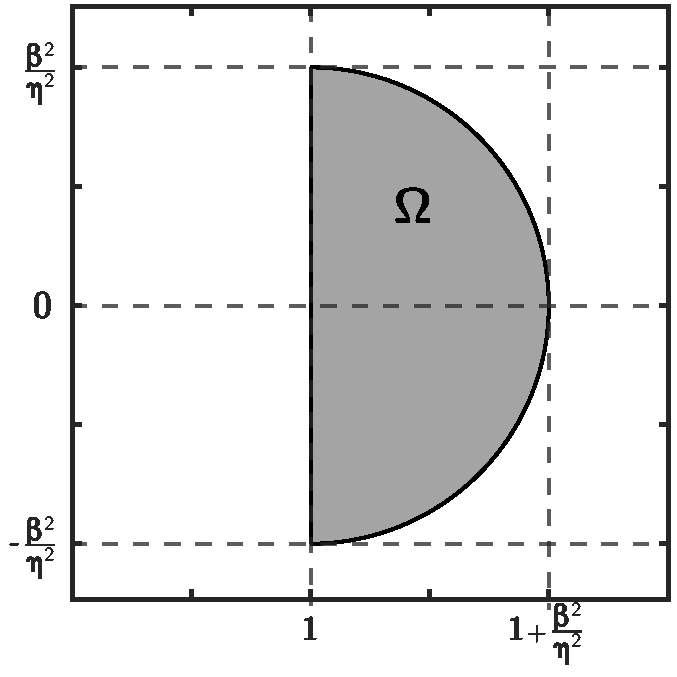
\includegraphics[width = 0.3\textwidth]{./figures/fov.pdf}
\caption{}
\label{fig:bound}
\end{figure}
\end{theorem}
%

% ------------------------------------------------------------------------------------- %
% ------------------------------------------------------------------------------------- %
\subsection{Conditioning}\label{sec:theory:cond}

Consider the Schur complement for two operators,
%
\begin{align}\label{eq:Schur}
S & := \eta I - \widehat{\mathcal{L}}_2 + \beta^2 (\eta I - \widehat{\mathcal{L}}_1)^{-1} \\
& = \left[\left(\eta I - \widehat{\mathcal{L}}_2\right)\left(\eta I - \widehat{\mathcal{L}}_1\right)
	+ \beta^2 I\right]\left(\eta I - \widehat{\mathcal{L}}_1\right)^{-1} \label{eq:Schur1}\\
& = \left(\eta I - \widehat{\mathcal{L}}_1\right)^{-1} \left[\left(\eta I - \widehat{\mathcal{L}}_1\right)
	\left(\eta I - \widehat{\mathcal{L}}_2\right) + \beta^2 I\right]. \label{eq:Schur2}
\end{align}



%
\begin{theorem}[Conditioning of preconditioned operator]\label{th:cond}
Suppose Assumptions \ref{ass:eig} and \ref{ass:fov} hold, that is, $\eta > 0$
and $W(\mathcal{L}) \leq 0$ \eqref{eq:fov}. Let $\eta \leq \gamma \leq \
\tfrac{\eta^2+\beta^2}{\eta}$ and let
$\mathcal{P}_\gamma$ denote the preconditioned operator, where $((\eta + i\beta)I -
\widehat{\mathcal{L}})((\eta - i\beta)I - \widehat{\mathcal{L}})$ is
preconditioned with $(\gamma I - \widehat{\mathcal{L}})^{-2}$. Then,
\begin{align}\label{eq:cond1}
\textnormal{cond}(\mathcal{P}_\gamma) \leq (1 + \alpha\overline{\alpha})
		\left(1 + \frac{\alpha\overline{\alpha}}{(1 - \alpha)(1 - \overline{\alpha})}\right)
	% \begin{cases} 
	% \frac{1 + \alpha\overline{\alpha}} {(1 - \alpha)(1 - \overline{\alpha})}
	% 	& \eta\gamma \geq \eta^2+\beta^2, \\
	% (1 + \alpha\overline{\alpha})
	% 	\left(1 + \frac{\alpha\overline{\alpha}}{(1 - \alpha)(1 - \overline{\alpha})}\right)
	% 	& \eta\gamma < \eta^2+\beta^2,
	% \end{cases}
\end{align}
with $\alpha$ and $\overline{\alpha}$ defined as in \eqref{eq:alpha}.
\end{theorem}
\begin{proof}
The proof proceeds as follows: first, we factor $\mathcal{P}_\gamma$ \eqref{eq:prec_k},
and proceed to use the factored form to derive an upper bound on 
$\|\mathcal{P}_\gamma\|$ and $\|\mathcal{P}_\gamma^{-1}\|$, which immediately
yields a bound on
%
\begin{align}\label{eq:cond0}
\textnormal{cond}(\mathcal{P}_\gamma) = \|\mathcal{P}_\gamma\|\|\mathcal{P}_\gamma^{-1}\|.
\end{align}
%
Note that following from the discussion in \Cref{sec:solve:inv} and \Cref{th:fov},
for real $k>0$, $W\left[\left(I - \tfrac{1}{k}\mathcal{L}\right)^{-1}\right]$ and
$W\left[\left(I - \tfrac{1}{k}\mathcal{L}\right)^{-2}\right]$ are contained in
the positive half unit circle, and $\|(I - \tfrac{1}{\gamma}\mathcal{L})^{-1}\| \leq 1$
(see proof of \Cref{th:fov}).

We start with $\|\mathcal{P}_\gamma\|$, where
%
\begin{align}\label{eq:CS}
\|\mathcal{P}_\gamma\| & \leq 
	\Big\|I - \overline{\alpha}\left(I - \tfrac{1}{\gamma}\mathcal{L}\right)^{-1}\Big\|
	\Big\|I - \alpha\left(I - \tfrac{1}{\gamma}\mathcal{L}\right)^{-1}\Big\|.
\end{align}
%
Recalling that $W\left[(I - \tfrac{1}{k}\mathcal{L})^{-1}\right] \geq 0$
and $\|(I - \tfrac{1}{\gamma}\mathcal{L})^{-1}\| \leq 1$, and using the
assumption $\gamma \geq \eta$, we can expand the norm squared in inner-product
form, yielding
%
\begin{align*}
&\hspace{-5ex}
\Big\|I - \overline{\alpha}\left(I - \tfrac{1}{\gamma}\mathcal{L}\right)^{-1}\Big\|^2 \\
	& = 1 + \max_{\mathbf{x}\neq\mathbf{0}} \left( \alpha\overline{\alpha}
		\frac{\left\|\left(I - \tfrac{1}{\gamma}\mathcal{L}\right)^{-1}\mathbf{x}\right\|^2
		}{\|\mathbf{x}\|^2}
	- (\alpha + \overline{\alpha})\frac{\textnormal{Re}\left(\left\langle\left(I -
		\tfrac{1}{\gamma}\mathcal{L}\right)^{-1}\mathbf{x}, \mathbf{x}\right\rangle\right)}
		{\|\mathbf{x}\|^2}\right) \\
& \leq 1 + \alpha\overline{\alpha}\left\|\left(I - \tfrac{1}{\gamma}\mathcal{L}\right)^{-1}\right\|^2 \\
& \leq 1 + \alpha\overline{\alpha}.
\end{align*}
%
Note that the above derivation is identical for $\alpha$ and $\overline{\alpha}$,
which yields
%
\begin{align} \label{eq:upper_alpha}
\|\mathcal{P}_\gamma\| & \leq 1 + \alpha\overline{\alpha}.
\end{align}
%

To bound $\|\mathcal{P}_\gamma^{-1}\|$, we use an analogous approach as above
\eqref{eq:CS}, developing bounds on the two polynomial factors separately.
First, note that
%
\begin{align}\nonumber
\left[I - \alpha\left(I - \tfrac{1}{\gamma}\mathcal{L}\right)^{-1}\right]^{-1}
	& = \left(I - \tfrac{1}{\gamma}\mathcal{L}\right)
		\left[(1-\alpha)I - \tfrac{1}{\gamma}\mathcal{L}\right]^{-1} \nonumber\\
& = \left[\alpha I + ((1-\alpha)I - \tfrac{1}{\gamma}\mathcal{L})\right]
		\left[(1-\alpha)I - \tfrac{1}{\gamma}\mathcal{L}\right]^{-1} \nonumber\\
& = I + \alpha \left[(1-\alpha)I - \tfrac{1}{\gamma}\mathcal{L}\right]^{-1} \nonumber\\
& = I + \frac{\alpha}{1-\alpha} \left(I - \tfrac{1}{\gamma(1-\alpha)}\mathcal{L}\right)^{-1}.
	\label{eq:inv_factor}
\end{align}
%
For condensed notation, let $c_\alpha := \tfrac{\alpha}{1-\alpha}$, and note that 
%
\begin{align*} 
c_\alpha+\overline{c_\alpha} & = \frac{\alpha + \overline{\alpha} - 2\alpha\overline{\alpha}}
	{1 + \alpha\overline{\alpha} - (\alpha + \overline{\alpha})} 
= \frac{2\eta\gamma - 2(\eta^2+\beta^2)}{\eta^2+\beta^2},
\end{align*}
%
which is $< 0$ when $\eta\gamma \leq (\eta^2+\beta^2)$ and $<0$ otherwise. 

Expanding the squared norm of \eqref{eq:inv_factor} in inner-product form, we have
%
\begin{align}\label{eq:pinv0}
& \hspace{-5ex}
1 + \max_{\mathbf{x}\neq\mathbf{0}} \left[ (c_\alpha+\overline{c_\alpha})
	\frac{\textnormal{Re}\left(\left\langle (I - \tfrac{1}{\gamma(1-\alpha)}\mathcal{L})^{-1}\mathbf{x},
		\mathbf{x}\right\rangle\right)}{\|\mathbf{x}\|^2} + 
	c_\alpha\overline{c_\alpha}
	\frac{\left\|(I - \tfrac{1}{\gamma(1-\alpha)}\mathcal{L})^{-1}\mathbf{x}\right\|^2}
		{\|\mathbf{x}\|^2} \right].
\end{align}
%
Bounding the norm term in \eqref{eq:pinv0} requires care because $\alpha$ is
complex. Note that the norm is the maximum singular value, which is equivalent to one
over the minimum nonzero singular value of the inverse. The squared minimum nonzero
singular value of the inverse of the inverse is given by
%
\begin{align*}
&\hspace{-5ex}
\min_{\mathbf{x}\neq\mathbf{0}} \frac{\left\|\left(I - \tfrac{1}{\gamma(1-\alpha)}
	\mathcal{L}\right)\mathbf{x}\right\|^2}{\|\mathbf{x}\|^2} \\
& = 1 + \min_{\mathbf{x}\neq\mathbf{0}} \left[ \frac{1}{|\gamma(1-\alpha)|^2}
	\frac{\left\|\mathcal{L}\mathbf{x}\right\|^2}{\|\mathbf{x}\|^2}
	- \left(\frac{1}{\gamma(1-\alpha)} + \frac{1}{\overline{\gamma}(1-\overline{\alpha})}\right)
	\frac{\textnormal{Re}\left(\left\langle\mathcal{L}\mathbf{x},\mathbf{x}\right\rangle\right)}
		{\|\mathbf{x}\|^2}\right].
\end{align*}
%
Noting that Re$\left(\langle\mathcal{L}\mathbf{x},\mathbf{x}\rangle\right) \leq 0$,
$\gamma \geq \eta > 0$, and Re$(1-\alpha) \geq 0$, it follows that the squared minimum
singular value above is $\geq 1$, which implies $\|(I - \tfrac{1}{\gamma(1-\alpha)}
\mathcal{L})^{-1}\| \leq 1$.

% ------> Old extra derivation for \gamma larger than currently considered
% ------------------------------------------------------------------------
% Plugging into \eqref{eq:pinv1} and noting
% that an identical derivation and result holds for $\overline{\alpha}$, we have
% for $(c_\alpha+\overline{c_\alpha}) \geq 0$,
% %
% \begin{align}\nonumber
% \|\mathcal{P}_\gamma^{-1}\| & \leq 
% 	\Big\|\Big(I - \overline{\alpha}\left(I - \tfrac{1}{\gamma}\mathcal{L}\right)^{-1}\Big)^{-1}\Big\|
% 	\Big\|\Big(I - \alpha\left(I - \tfrac{1}{\gamma}\mathcal{L}\right)^{-1}\Big)^{-1}\Big\| \\
% & \leq \left(1 + \frac{\alpha}{1-\alpha}\right)
% 	\left(1 + \frac{\overline{\alpha}}{1-\overline{\alpha}}\right) \nonumber\\
% & = \frac{1}{(1 - \alpha)(1 - \overline{\alpha})}. \label{eq:lower_alpha1}
% \end{align}
% %

Returning to \eqref{eq:pinv0}, consider the inner-product term with leading
constant $(c_\alpha+\overline{c_\alpha}) \leq 0$. Note that letting
$\mathbf{x}:= (I - \tfrac{1}{\gamma(1-\alpha)}\mathcal{L})\mathbf{y}$,
we have
%
\begin{align*}
\frac{\left\langle (I - \tfrac{1}{\gamma(1-\alpha)}\mathcal{L})^{-1}\mathbf{x},
		\mathbf{x}\right\rangle}{\|\mathbf{x}\|^2}
& = \frac{\left\langle \mathbf{y}, (I - \tfrac{1}{\gamma(1-\alpha)}\mathcal{L})\mathbf{y}
	\right\rangle}{\|(I - \tfrac{1}{\gamma(1-\alpha)}\mathcal{L})\mathbf{y}\|^2}
= \frac{\|\mathbf{y}\|^2 - \frac{1}{\gamma (1 - \overline{\alpha})}
	\left\langle \mathbf{y},\mathcal{L}\mathbf{y} \right\rangle}
	{\|(I - \tfrac{1}{\gamma(1-\alpha)}\mathcal{L})\mathbf{y}\|^2}.
\end{align*}
%
By assumption, Re$\left(\langle \mathbf{y},\mathcal{L}\mathbf{y}\rangle\right) \leq 0$,
while $\gamma\geq 0$ and Re$(1-\alpha) \geq 0$. It follows that
%
\begin{align*}
\textnormal{Re}\left(\frac{\left\langle (I - \tfrac{1}{\gamma(1-\alpha)}\mathcal{L})^{-1}\mathbf{x},
	\mathbf{x}\right\rangle}{\|\mathbf{x}\|^2}\right) \geq 0.
\end{align*}
%
Thus in \eqref{eq:pinv0} because $(c_\alpha+\overline{c_\alpha}) \leq 0$, we can drop
the corresponding term for an upper bound of
%
\begin{align*}
\left\|\left[I - \alpha\left(I - \tfrac{1}{\gamma}\mathcal{L}\right)^{-1}\right]^{-1}\right\|^2 
	& \leq 1 + c_\alpha\overline{c_\alpha}
		\left\|(I - \tfrac{1}{\gamma(1-\alpha)}\mathcal{L})^{-1}\right\|^2 \\
& \leq 1 + c_\alpha\overline{c_\alpha} \\
& = 1 + \frac{\alpha\overline{\alpha}}{(1 - \alpha)(1 - \overline{\alpha})}.
\end{align*}
%
Again noting that analogous derivations holds for $\overline{\alpha}$ with
identical bounds, we have for $(c_\alpha+\overline{c_\alpha}) < 0$,
%
\begin{align}
\|\mathcal{P}_\gamma^{-1}\| & \leq 1 + 
	\frac{\alpha\overline{\alpha}}{(1 - \alpha)(1 - \overline{\alpha})}. \label{eq:lower_alpha2}
\end{align}
% 

Combining \eqref{eq:cond0}, \eqref{eq:upper_alpha},
and \eqref{eq:lower_alpha2} completes the proof.
\end{proof}
%



%
\begin{corollary}[Conditioning independent of $\eta$ and $\beta$]\label{cor:independent}
Preconditioning $\mathcal{Q}_\eta$ \eqref{eq:imag1} with
$(\gamma_* I - \widehat{\mathcal{L}})^{-2}$, 

\begin{align}\label{eq:cond_eta}
\textnormal{cond}(\mathcal{P}_{\gamma = \eta}) & \leq 1 + 2\frac{\beta^2}{\eta^2}, \\
\textnormal{cond}(\mathcal{P}_{\gamma_*}) & \leq
	\left(3 - 2\frac{\eta}{\sqrt{\eta^2+\beta^2}}\right)^2, \\
\textnormal{cond}\left(\mathcal{P}_{\gamma = \frac{\eta^2+\beta^2}{\eta}}\right) & \leq
	\left(1 + \frac{\beta^2}{\eta^2}\right) \left(1 + \frac{\beta^2}{\beta^2 + \eta^2}\right), \\
\end{align}

\end{corollary}
%
It is also worth pointing out that as $\beta \to 0$, $\gamma \to \eta$
in all three of the above cases, and (as expected) \eqref{eq:cond_eta},
\eqref{eq:cond_upper}, and \eqref{eq:cond_opt} all $\to 1$.


% ------------------------------------------------------------------------------------- %
% ------------------------------------------------------------------------------------- %
% ------------------------------------------------------------------------------------- %
\section{Differential algebraic equations}\label{sec:dae}



% ------------------------------------------------------------------------------------- %
% ------------------------------------------------------------------------------------- %
% ------------------------------------------------------------------------------------- %
\section{Numerical results}\label{sec:numerics_nonlin}

% ------------------------------------------------------------------------------------- %
% ------------------------------------------------------------------------------------- %
\subsection{Nonlinear advection-diffusion}\label{sec:numerics_nonlin:advdiff}



% ------------------------------------------------------------------------------------- %
% ------------------------------------------------------------------------------------- %
\subsection{Nonlinear heat conduction}\label{sec:numerics_nonlin:heat}

Consider Example 16p in MFEM, which solves a nonlinear heat conduction equation
%
\begin{align*}
u_t  & = \nabla\cdot (\kappa + \alpha u) \nabla u.
\end{align*}
%
Let us express the diffusion as a nonlinear matrix-valued operator $K(u)$ with
potential forcing function $f(t)$. Discretizing in space we can express the semidiscrete 
system as the nonlinear set of equations
%
\begin{align*}
M\mathbf{u}_t & = K(\mathbf{u})\mathbf{u} + \mathbf{f}.
\end{align*}
%
Here we demonstrate how a typical Picard linearization can fit into the 
framework developed above. Let $\mathbf{u}_i$ denote $\mathbf{u}$ at the $i$th
time step, and consider a backward Euler step,
%
\begin{align*}
M\mathbf{u}_{i+1} & = M\mathbf{u}_i + \delta tK(\mathbf{u}_{i+1}) + \mathbf{f}.
\end{align*}
%
Rearranging yields a nonlinear system $\mathcal{F}(\mathbf{u}_{i+1}) = \mathbf{0}$,
where
%
\begin{align*}
\mathcal{F}(\mathbf{u}_{i+1}) := 
	(M - \delta t K(\mathbf{u}_{i+1}))\mathbf{u}_{i+1} - M\mathbf{u}_i - \mathbf{f}.
\end{align*}
%
We can invert the matrix-valued operator as a linear preconditioning, leading
to an equivalent nonlinear system $\mathcal{H}(\mathbf{u}_{i+1}) = \mathbf{0}$,
where
%
\begin{align*}
\mathcal{H}(\mathbf{u}_{i+1}) := 
	(M - \delta t K(\mathbf{u}_{i+1}))^{-1}(M\mathbf{u}_i + \mathbf{f}) - \mathbf{u}_{i+1}.
\end{align*}
%
Finally, we formulate a Picard iteration by defining $\mathcal{G}(\mathbf{u}_{i+1}) :=
\mathcal{H}(\mathbf{u}_{i+1}) + \mathbf{u}_{i+1}$, and noting that
$\mathbf{G}(\mathbf{u}_{i+1}) = \mathbf{u}_{i+1}$ if and only if
$\mathcal{F}(\mathbf{u}_{i+1}) = \mathbf{0}$. Fixed-point iterations are then
given by 
%
\begin{align*}
\mathbf{u}_{i+1}^{k+1} & = \mathcal{G}(\mathbf{u}_{i+1}^k) \\
& = (M - \delta t K(\mathbf{u}_{i+1}^k))^{-1}(M\mathbf{u}_i + \mathbf{f}), \\
\Longleftrightarrow\hspace{5ex}
(M - \delta t K(\mathbf{u}_{i+1}^k))\mathbf{u}_{i+1}^k& = M\mathbf{u}_i + \mathbf{f}.\
\end{align*}
%

In fact, this is exactly a Newton-like iteration approximating the Jacobian of
$\mathcal{F}(\mathbf{u}_{i+1})$ evaluated at $\mathbf{u}_{i+1}^k$ as
$J[\mathbf{u}_{i+1}^k] \approx (M - \delta t K(\mathbf{u}_{i+1}^k))$. We use
this observation to extend the same principle to IRK methods, approximating
the Jacobian for the stage equations \eqref{eq:stages} evaluated at the previous
stage vectors as
%
\begin{align*}
&J[\mathbf{k}_1^{k},...,\mathbf{k}_s^k] \approx \\
&\begin{bmatrix} M \\ & \ddots & \\ && M \end{bmatrix} - \delta t
	\begin{bmatrix} a_{11}K\left(\mathbf{u}_n + \delta t\sum_{j=1}^s
	a_{1j}\mathbf{k}_j^k\right) & ... & a_{1s}K\left(\mathbf{u}_n + \delta t\sum_{j=1}^s
	a_{ij}\mathbf{k}_j^k\right) \\
	\vdots & \ddots & \vdots \\
	a_{s1}K\left(\mathbf{u}_n + \delta t\sum_{j=1}^s
	a_{sj}\mathbf{k}_j^k\right) & ... & a_{ss}K\left(\mathbf{u}_n + \delta t\sum_{j=1}^s
	a_{sj}\mathbf{k}_j^k\right)
	\end{bmatrix}.
\end{align*}
%
Letting $\mathcal{L}_i := K\left(\mathbf{u}_n + \delta t\sum_{j=1}^s
a_{ij}\mathbf{k}_j^k\right)$ denote the approximate jacobian for the
$i$th row, we can proceed exactly as discussed in \Cref{sec:nonlinear}.

%
\begin{remark}[Picard as a Newton-like method]
Note, it is important to express Picard and fixed-point iterations in the 
form of a Newton-like method to use the preconditioning techniques developed
in this paper! By expressing it as a Newton-like method, we are approximating
the Jacobian and will still converge to the solution of the nonlinear functional
$\mathcal{F} = 0$ when adding levels of approximation as in \Cref{sec:nonlinear:gen}.
A traditional Picard iteration relies on converging exactly to the fixed-point
$\mathcal{G}(\mathbf{k}) = \mathbf{k}$ via iterates $\mathbf{k}^{k+1} =
\mathcal{G}(\mathbf{k}^k)$. Within this iteration there is delicate cancellation
that result from solving directly for $\mathbf{k}^{k+1}$ rather than a correction,
and approximating $\mathcal{G}$ would result in convergence to a different problem.
\end{remark}
%

% ------------------------------------------------------------------------------------- %
% ------------------------------------------------------------------------------------- %
\subsection{Compressible Navier Stokes}\label{sec:numerics_nonlin:ns}





% ------------------------------------------------------------------------------------- %
% ------------------------------------------------------------------------------------- %
% ------------------------------------------------------------------------------------- %
\section{Conclusions}\label{sec:conc}

This paper introduced a theoretical and algorithmic framework for the fast, parallel
solution of fully implicit Runge-Kutta methods in numerical PDEs (without algebraic
constraints). A field-of-values analysis is derived to guarantee rapid Krylov
convergence...\todo{finish}


% % ------------------------------------------------------------------------------------- %
% % ------------------------------------------------------------------------------------- %
% % ------------------------------------------------------------------------------------- %
% \section*{Appendix}

% % ------------------------------------------------------------------------------------- %
% % ------------------------------------------------------------------------------------- %
% \subsection{Real Schur decomposition applied to general operators}

% Here we write out $(Q_0^T\otimes I)\boldsymbol{\mathcal{L}}(Q_0\otimes I)$
% in bracket notation, where, e.g., $\{a_1,a_2,a_3\}\mapsto a_1\mathcal{L}_1 + a_2\mathcal{L}_2 + 
% a_3\mathcal{L}_3$. Note in the matrices below, the constants in diagonal brackets always
% sum to one and off-diagonal sum to zero, wherein if $\mathcal{L}_i = \mathcal{L}_j$ for
% all $i,j$, each of the following operators is the identity.

% % ------------------------------------------------------------------------------------- %
% \subsubsection*{Gauss}

% %
% \textbf{2-stage:}
% \begin{align*}
% \begin{bmatrix}
% \{1,0\} & \{0,0\} \\
%  \{0,0\} & \{0,1\} \\
% \end{bmatrix}
% \end{align*}
% %
% \textbf{3,-stage:}
% \begin{align*}
% \begin{bmatrix}
% \{0.002,0.565,0.432\} & \{-0.038,-0.245,0.284\} & \{0.024,-0.430,0.405\}\\
% \{-0.038,-0.245,0.284\} & \{0.705,0.107,0.187\} & \{-0.453,0.187,0.266\}\\
% \{0.024,-0.430,0.405\} & \{-0.453,0.187,0.266\} & \{0.291,0.327,0.380\}\\
% \end{bmatrix}
% \end{align*}
% %
% \textbf{4,-stage:}
% \begin{align*}
% \begin{bmatrix}
% \{0.002,0.014,0.012,0.970\} & \{0.001,-0.011,-0.110,0.120\} & \{-0.016,-0.113,0.010,0.119\} & \{-0.045,0.041,-0.005,0.009\}\\
% \{0.001,-0.011,-0.110,0.120\} & \{0.000,0.008,0.975,0.014\} & \{-0.007,0.085,-0.093,0.014\} & \{-0.021,-0.031,0.051,0.001\}\\
% \{-0.016,-0.113,0.010,0.119\} & \{-0.007,0.085,-0.093,0.014\} & \{0.113,0.863,0.008,0.014\} & \{0.316,-0.312,-0.004,0.001\}\\
% \{-0.045,0.041,-0.005,0.009\} & \{-0.021,-0.031,0.051,0.001\} & \{0.316,-0.312,-0.004,0.001\} & \{0.883,0.113,0.002,0.000\}\\
% \end{bmatrix}
% \end{align*}


% %,-,-,-,-,-,-,-,-,-,-,-,-,-,-,-,-,-,-,-,-,-,-,-,-,-,-,-,-,-,-,-,-,-,-,-,-,-,-,-,-,-,-,-,-,-,-,-,-,-,-,-,-,-,-,-,-,-,-,-,-,-,-,-,-,-,-,-,-,-,-,-,-,-,-,-,-,-,-,-,-,-,-,-,-,-%
% \subsubsection*{RadauIIA}

% %
% \textbf{2,-stage:}
% \begin{align*}
% \begin{bmatrix}
% \{0.985,0.014\} & \{0.121,-0.121\}\\
% \{0.121,-0.121\} & \{0.014,0.985\}\\
% \end{bmatrix}
% \end{align*}
% %
% \textbf{3,-stage:}
% \begin{align*}
% \begin{bmatrix}
% \{0.019,0.052,0.928\} & \{0.006,0.222,-0.229\} & \{0.137,-0.017,-0.119\}\\
% \{0.006,0.222,-0.229\} & \{0.002,0.941,0.056\} & \{0.045,-0.075,0.029\}\\
% \{0.137,-0.017,-0.119\} & \{0.045,-0.075,0.029\} & \{0.978,0.006,0.015\}\\
% \end{bmatrix}
% \end{align*}
% %
% \textbf{4,-stage:}
% \begin{align*}
% \begin{bmatrix}
% \{0.002,0.031,0.103,0.862\} & \{0.006,0.022,-0.301,0.272\} & \{0.052,-0.049,0.025,-0.028\} & \{-0.014,-0.166,-0.029,0.209\}\\
% \{0.006,0.022,-0.301,0.272\} & \{0.015,0.016,0.882,0.085\} & \{0.120,-0.035,-0.075,-0.009\} & \{-0.032,-0.118,0.084,0.066\}\\
% \{0.052,-0.049,0.025,-0.028\} & \{0.120,-0.035,-0.075,-0.009\} & \{0.915,0.077,0.006,0.000\} & \{-0.245,0.260,-0.007,-0.006\}\\
% \{-0.014,-0.166,-0.029,0.209\} & \{-0.032,-0.118,0.084,0.066\} & \{-0.245,0.260,-0.007,-0.006\} & \{0.066,0.874,0.008,0.050\}\\
% \end{bmatrix}
% \end{align*}

% ------------------------------------------------------------------------------- %
\bibliographystyle{siamplain}
\bibliography{refs2.bib}


\end{document}


ADJUGATE FORMS, b^T * A0^{-1} * Adj(Ms)
Let M = A0^{-1}, with entries {m_ij}, b = b[b1,...,bs], and xx = spatial operator L

Stiffly accurate RK (b0^TA0^{-1} = [0,...,0,1])
-----------------------------------------------
s = 2
  -m21,
  m11 - xx

s = 3
  -m22 m31 + m21 m32 + m31 xx, 
  m12 m31 - m11 m32 + m32 xx,
  -m12 m21 + m11 m22 - m11 xx - m22 xx + xx^2

s = 4
  m23 m32 m41 - m22 m33 m41 - m23 m31 m42 + m21 m33 m42 + m22 m31 m43 - 
	 m21 m32 m43 + m22 m41 xx + m33 m41 xx - m21 m42 xx - m31 m43 xx - 
	 m41 xx^2,
  -m13 m32 m41 + m12 m33 m41 + m13 m31 m42 - m11 m33 m42 - 
	 m12 m31 m43 + m11 m32 m43 - m12 m41 xx + m11 m42 xx + m33 m42 xx - 
	 m32 m43 xx - m42 xx^2, 
  m13 m22 m41 - m12 m23 m41 - m13 m21 m42 + m11 m23 m42 + m12 m21 m43 - 
	 m11 m22 m43 - m13 m41 xx - m23 m42 xx + m11 m43 xx + m22 m43 xx - 
	 m43 xx^2,
  -m13 m22 m31 + m12 m23 m31 + m13 m21 m32 - m11 m23 m32 - 
	 m12 m21 m33 + m11 m22 m33 + m12 m21 xx - m11 m22 xx + m13 m31 xx + 
	 m23 m32 xx - m11 m33 xx - m22 m33 xx + m11 xx^2 + m22 xx^2 + 
	 m33 xx^2 - xx^3

s = 5
  m24 m33 m42 m51 - m23 m34 m42 m51 - m24 m32 m43 m51 + 
	  m22 m34 m43 m51 + m23 m32 m44 m51 - m22 m33 m44 m51 - 
	  m24 m33 m41 m52 + m23 m34 m41 m52 + m24 m31 m43 m52 - 
	  m21 m34 m43 m52 - m23 m31 m44 m52 + m21 m33 m44 m52 + 
	  m24 m32 m41 m53 - m22 m34 m41 m53 - m24 m31 m42 m53 + 
	  m21 m34 m42 m53 + m22 m31 m44 m53 - m21 m32 m44 m53 - 
	  m23 m32 m41 m54 + m22 m33 m41 m54 + m23 m31 m42 m54 - 
	  m21 m33 m42 m54 - m22 m31 m43 m54 + m21 m32 m43 m54 - 
	  m23 m32 m51 xx + m22 m33 m51 xx - m24 m42 m51 xx - m34 m43 m51 xx + 
	  m22 m44 m51 xx + m33 m44 m51 xx + m23 m31 m52 xx - m21 m33 m52 xx + 
	  m24 m41 m52 xx - m21 m44 m52 xx - m22 m31 m53 xx + m21 m32 m53 xx + 
	  m34 m41 m53 xx - m31 m44 m53 xx - m22 m41 m54 xx - m33 m41 m54 xx + 
	  m21 m42 m54 xx + m31 m43 m54 xx - m22 m51 xx^2 - m33 m51 xx^2 - 
	  m44 m51 xx^2 + m21 m52 xx^2 + m31 m53 xx^2 + m41 m54 xx^2 + 
	  m51 xx^3,
  -m14 m33 m42 m51 + m13 m34 m42 m51 + m14 m32 m43 m51 - 
	  m12 m34 m43 m51 - m13 m32 m44 m51 + m12 m33 m44 m51 + 
	  m14 m33 m41 m52 - m13 m34 m41 m52 - m14 m31 m43 m52 + 
	  m11 m34 m43 m52 + m13 m31 m44 m52 - m11 m33 m44 m52 - 
	  m14 m32 m41 m53 + m12 m34 m41 m53 + m14 m31 m42 m53 - 
	  m11 m34 m42 m53 - m12 m31 m44 m53 + m11 m32 m44 m53 + 
	  m13 m32 m41 m54 - m12 m33 m41 m54 - m13 m31 m42 m54 + 
	  m11 m33 m42 m54 + m12 m31 m43 m54 - m11 m32 m43 m54 + 
	  m13 m32 m51 xx - m12 m33 m51 xx + m14 m42 m51 xx - m12 m44 m51 xx - 
	  m13 m31 m52 xx + m11 m33 m52 xx - m14 m41 m52 xx - m34 m43 m52 xx + 
	  m11 m44 m52 xx + m33 m44 m52 xx + m12 m31 m53 xx - m11 m32 m53 xx + 
	  m34 m42 m53 xx - m32 m44 m53 xx + m12 m41 m54 xx - m11 m42 m54 xx - 
	  m33 m42 m54 xx + m32 m43 m54 xx + m12 m51 xx^2 - m11 m52 xx^2 - 
	  m33 m52 xx^2 - m44 m52 xx^2 + m32 m53 xx^2 + m42 m54 xx^2 + 
	  m52 xx^3, 
  m14 m23 m42 m51 - m13 m24 m42 m51 - m14 m22 m43 m51 + 
	  m12 m24 m43 m51 + m13 m22 m44 m51 - m12 m23 m44 m51 - 
	  m14 m23 m41 m52 + m13 m24 m41 m52 + m14 m21 m43 m52 - 
	  m11 m24 m43 m52 - m13 m21 m44 m52 + m11 m23 m44 m52 + 
	  m14 m22 m41 m53 - m12 m24 m41 m53 - m14 m21 m42 m53 + 
	  m11 m24 m42 m53 + m12 m21 m44 m53 - m11 m22 m44 m53 - 
	  m13 m22 m41 m54 + m12 m23 m41 m54 + m13 m21 m42 m54 - 
	  m11 m23 m42 m54 - m12 m21 m43 m54 + m11 m22 m43 m54 - 
	  m13 m22 m51 xx + m12 m23 m51 xx + m14 m43 m51 xx - m13 m44 m51 xx + 
	  m13 m21 m52 xx - m11 m23 m52 xx + m24 m43 m52 xx - m23 m44 m52 xx - 
	  m12 m21 m53 xx + m11 m22 m53 xx - m14 m41 m53 xx - m24 m42 m53 xx + 
	  m11 m44 m53 xx + m22 m44 m53 xx + m13 m41 m54 xx + m23 m42 m54 xx - 
	  m11 m43 m54 xx - m22 m43 m54 xx + m13 m51 xx^2 + m23 m52 xx^2 - 
	  m11 m53 xx^2 - m22 m53 xx^2 - m44 m53 xx^2 + m43 m54 xx^2 + 
	  m53 xx^3,
  -m14 m23 m32 m51 + m13 m24 m32 m51 + m14 m22 m33 m51 - 
	  m12 m24 m33 m51 - m13 m22 m34 m51 + m12 m23 m34 m51 + 
	  m14 m23 m31 m52 - m13 m24 m31 m52 - m14 m21 m33 m52 + 
	  m11 m24 m33 m52 + m13 m21 m34 m52 - m11 m23 m34 m52 - 
	  m14 m22 m31 m53 + m12 m24 m31 m53 + m14 m21 m32 m53 - 
	  m11 m24 m32 m53 - m12 m21 m34 m53 + m11 m22 m34 m53 + 
	  m13 m22 m31 m54 - m12 m23 m31 m54 - m13 m21 m32 m54 + 
	  m11 m23 m32 m54 + m12 m21 m33 m54 - m11 m22 m33 m54 - 
	  m14 m22 m51 xx + m12 m24 m51 xx - m14 m33 m51 xx + m13 m34 m51 xx + 
	  m14 m21 m52 xx - m11 m24 m52 xx - m24 m33 m52 xx + m23 m34 m52 xx + 
	  m14 m31 m53 xx + m24 m32 m53 xx - m11 m34 m53 xx - m22 m34 m53 xx - 
	  m12 m21 m54 xx + m11 m22 m54 xx - m13 m31 m54 xx - m23 m32 m54 xx + 
	  m11 m33 m54 xx + m22 m33 m54 xx + m14 m51 xx^2 + m24 m52 xx^2 + 
	  m34 m53 xx^2 - m11 m54 xx^2 - m22 m54 xx^2 - m33 m54 xx^2 + 
	  m54 xx^3, 
  m14 m23 m32 m41 - m13 m24 m32 m41 - m14 m22 m33 m41 + 
	  m12 m24 m33 m41 + m13 m22 m34 m41 - m12 m23 m34 m41 - 
	  m14 m23 m31 m42 + m13 m24 m31 m42 + m14 m21 m33 m42 - 
	  m11 m24 m33 m42 - m13 m21 m34 m42 + m11 m23 m34 m42 + 
	  m14 m22 m31 m43 - m12 m24 m31 m43 - m14 m21 m32 m43 + 
	  m11 m24 m32 m43 + m12 m21 m34 m43 - m11 m22 m34 m43 - 
	  m13 m22 m31 m44 + m12 m23 m31 m44 + m13 m21 m32 m44 - 
	  m11 m23 m32 m44 - m12 m21 m33 m44 + m11 m22 m33 m44 + 
	  m13 m22 m31 xx - m12 m23 m31 xx - m13 m21 m32 xx + m11 m23 m32 xx + 
	  m12 m21 m33 xx - m11 m22 m33 xx + m14 m22 m41 xx - m12 m24 m41 xx + 
	  m14 m33 m41 xx - m13 m34 m41 xx - m14 m21 m42 xx + m11 m24 m42 xx + 
	  m24 m33 m42 xx - m23 m34 m42 xx - m14 m31 m43 xx - m24 m32 m43 xx + 
	  m11 m34 m43 xx + m22 m34 m43 xx + m12 m21 m44 xx - m11 m22 m44 xx + 
	  m13 m31 m44 xx + m23 m32 m44 xx - m11 m33 m44 xx - m22 m33 m44 xx - 
	  m12 m21 xx^2 + m11 m22 xx^2 - m13 m31 xx^2 - m23 m32 xx^2 + 
	  m11 m33 xx^2 + m22 m33 xx^2 - m14 m41 xx^2 - m24 m42 xx^2 - 
	  m34 m43 xx^2 + m11 m44 xx^2 + m22 m44 xx^2 + m33 m44 xx^2 - 
	  m11 xx^3 - m22 xx^3 - m33 xx^3 - m44 xx^3 + xx^4

Full implicit RK
----------------
s = 2
  -b1 m12 m21 + b1 m11 m22 - b1 m11 xx - b2 m21 xx,
  -b2 m12 m21 + b2 m11 m22 - b1 m12 xx - b2 m22 xx

s = 3
  -b1 m13 m22 m31 + b1 m12 m23 m31 + b1 m13 m21 m32 - b1 m11 m23 m32 -
     b1 m12 m21 m33 + b1 m11 m22 m33 + b1 m12 m21 xx - b1 m11 m22 xx + 
     b1 m13 m31 xx - b3 m22 m31 xx + b2 m23 m31 xx + b3 m21 m32 xx - 
     b1 m11 m33 xx - b2 m21 m33 xx + b1 m11 xx^2 + b2 m21 xx^2 + 
     b3 m31 xx^2,
  -b2 m13 m22 m31 + b2 m12 m23 m31 + b2 m13 m21 m32 - 
     b2 m11 m23 m32 - b2 m12 m21 m33 + b2 m11 m22 m33 + b2 m12 m21 xx - 
     b2 m11 m22 xx + b3 m12 m31 xx - b3 m11 m32 xx + b1 m13 m32 xx + 
     b2 m23 m32 xx - b1 m12 m33 xx - b2 m22 m33 xx + b1 m12 xx^2 + 
     b2 m22 xx^2 + b3 m32 xx^2,
  -b3 m13 m22 m31 + b3 m12 m23 m31 + 
     b3 m13 m21 m32 - b3 m11 m23 m32 - b3 m12 m21 m33 + b3 m11 m22 m33 +
     b2 m13 m21 xx - b1 m13 m22 xx - b2 m11 m23 xx + b1 m12 m23 xx + 
     b3 m13 m31 xx + b3 m23 m32 xx - b3 m11 m33 xx - b3 m22 m33 xx + 
     b1 m13 xx^2 + b2 m23 xx^2 + b3 m33 xx^2

s = 4
  b1 m14 m23 m32 m41 - b1 m13 m24 m32 m41 - b1 m14 m22 m33 m41 + 
	  b1 m12 m24 m33 m41 + b1 m13 m22 m34 m41 - b1 m12 m23 m34 m41 - 
	  b1 m14 m23 m31 m42 + b1 m13 m24 m31 m42 + b1 m14 m21 m33 m42 - 
	  b1 m11 m24 m33 m42 - b1 m13 m21 m34 m42 + b1 m11 m23 m34 m42 + 
	  b1 m14 m22 m31 m43 - b1 m12 m24 m31 m43 - b1 m14 m21 m32 m43 + 
	  b1 m11 m24 m32 m43 + b1 m12 m21 m34 m43 - b1 m11 m22 m34 m43 - 
	  b1 m13 m22 m31 m44 + b1 m12 m23 m31 m44 + b1 m13 m21 m32 m44 - 
	  b1 m11 m23 m32 m44 - b1 m12 m21 m33 m44 + b1 m11 m22 m33 m44 + 
	  b1 m13 m22 m31 xx - b1 m12 m23 m31 xx - b1 m13 m21 m32 xx + 
	  b1 m11 m23 m32 xx + b1 m12 m21 m33 xx - b1 m11 m22 m33 xx + 
	  b1 m14 m22 m41 xx - b1 m12 m24 m41 xx + b4 m23 m32 m41 xx - 
	  b3 m24 m32 m41 xx + b1 m14 m33 m41 xx - b4 m22 m33 m41 xx + 
	  b2 m24 m33 m41 xx - b1 m13 m34 m41 xx + b3 m22 m34 m41 xx - 
	  b2 m23 m34 m41 xx - b1 m14 m21 m42 xx + b1 m11 m24 m42 xx - 
	  b4 m23 m31 m42 xx + b3 m24 m31 m42 xx + b4 m21 m33 m42 xx - 
	  b3 m21 m34 m42 xx - b1 m14 m31 m43 xx + b4 m22 m31 m43 xx - 
	  b2 m24 m31 m43 xx - b4 m21 m32 m43 xx + b1 m11 m34 m43 xx + 
	  b2 m21 m34 m43 xx + b1 m12 m21 m44 xx - b1 m11 m22 m44 xx + 
	  b1 m13 m31 m44 xx - b3 m22 m31 m44 xx + b2 m23 m31 m44 xx + 
	  b3 m21 m32 m44 xx - b1 m11 m33 m44 xx - b2 m21 m33 m44 xx - 
	  b1 m12 m21 xx^2 + b1 m11 m22 xx^2 - b1 m13 m31 xx^2 + 
	  b3 m22 m31 xx^2 - b2 m23 m31 xx^2 - b3 m21 m32 xx^2 + 
	  b1 m11 m33 xx^2 + b2 m21 m33 xx^2 - b1 m14 m41 xx^2 + 
	  b4 m22 m41 xx^2 - b2 m24 m41 xx^2 + b4 m33 m41 xx^2 - 
	  b3 m34 m41 xx^2 - b4 m21 m42 xx^2 - b4 m31 m43 xx^2 + 
	  b1 m11 m44 xx^2 + b2 m21 m44 xx^2 + b3 m31 m44 xx^2 - b1 m11 xx^3 - 
	  b2 m21 xx^3 - b3 m31 xx^3 - b4 m41 xx^3, 
   b2 m14 m23 m32 m41 - b2 m13 m24 m32 m41 - b2 m14 m22 m33 m41 + 
	  b2 m12 m24 m33 m41 + b2 m13 m22 m34 m41 - b2 m12 m23 m34 m41 - 
	  b2 m14 m23 m31 m42 + b2 m13 m24 m31 m42 + b2 m14 m21 m33 m42 - 
	  b2 m11 m24 m33 m42 - b2 m13 m21 m34 m42 + b2 m11 m23 m34 m42 + 
	  b2 m14 m22 m31 m43 - b2 m12 m24 m31 m43 - b2 m14 m21 m32 m43 + 
	  b2 m11 m24 m32 m43 + b2 m12 m21 m34 m43 - b2 m11 m22 m34 m43 - 
	  b2 m13 m22 m31 m44 + b2 m12 m23 m31 m44 + b2 m13 m21 m32 m44 - 
	  b2 m11 m23 m32 m44 - b2 m12 m21 m33 m44 + b2 m11 m22 m33 m44 + 
	  b2 m13 m22 m31 xx - b2 m12 m23 m31 xx - b2 m13 m21 m32 xx + 
	  b2 m11 m23 m32 xx + b2 m12 m21 m33 xx - b2 m11 m22 m33 xx + 
	  b2 m14 m22 m41 xx - b2 m12 m24 m41 xx - b4 m13 m32 m41 xx + 
	  b3 m14 m32 m41 xx + b4 m12 m33 m41 xx - b3 m12 m34 m41 xx - 
	  b2 m14 m21 m42 xx + b2 m11 m24 m42 xx + b4 m13 m31 m42 xx - 
	  b3 m14 m31 m42 xx - b4 m11 m33 m42 xx + b1 m14 m33 m42 xx + 
	  b2 m24 m33 m42 xx + b3 m11 m34 m42 xx - b1 m13 m34 m42 xx - 
	  b2 m23 m34 m42 xx - b4 m12 m31 m43 xx + b4 m11 m32 m43 xx - 
	  b1 m14 m32 m43 xx - b2 m24 m32 m43 xx + b1 m12 m34 m43 xx + 
	  b2 m22 m34 m43 xx + b2 m12 m21 m44 xx - b2 m11 m22 m44 xx + 
	  b3 m12 m31 m44 xx - b3 m11 m32 m44 xx + b1 m13 m32 m44 xx + 
	  b2 m23 m32 m44 xx - b1 m12 m33 m44 xx - b2 m22 m33 m44 xx - 
	  b2 m12 m21 xx^2 + b2 m11 m22 xx^2 - b3 m12 m31 xx^2 + 
	  b3 m11 m32 xx^2 - b1 m13 m32 xx^2 - b2 m23 m32 xx^2 + 
	  b1 m12 m33 xx^2 + b2 m22 m33 xx^2 - b4 m12 m41 xx^2 + 
	  b4 m11 m42 xx^2 - b1 m14 m42 xx^2 - b2 m24 m42 xx^2 + 
	  b4 m33 m42 xx^2 - b3 m34 m42 xx^2 - b4 m32 m43 xx^2 + 
	  b1 m12 m44 xx^2 + b2 m22 m44 xx^2 + b3 m32 m44 xx^2 - b1 m12 xx^3 - 
	  b2 m22 xx^3 - b3 m32 xx^3 - b4 m42 xx^3, 
   b3 m14 m23 m32 m41 - b3 m13 m24 m32 m41 - b3 m14 m22 m33 m41 + 
	  b3 m12 m24 m33 m41 + b3 m13 m22 m34 m41 - b3 m12 m23 m34 m41 - 
	  b3 m14 m23 m31 m42 + b3 m13 m24 m31 m42 + b3 m14 m21 m33 m42 - 
	  b3 m11 m24 m33 m42 - b3 m13 m21 m34 m42 + b3 m11 m23 m34 m42 + 
	  b3 m14 m22 m31 m43 - b3 m12 m24 m31 m43 - b3 m14 m21 m32 m43 + 
	  b3 m11 m24 m32 m43 + b3 m12 m21 m34 m43 - b3 m11 m22 m34 m43 - 
	  b3 m13 m22 m31 m44 + b3 m12 m23 m31 m44 + b3 m13 m21 m32 m44 - 
	  b3 m11 m23 m32 m44 - b3 m12 m21 m33 m44 + b3 m11 m22 m33 m44 + 
	  b3 m13 m22 m31 xx - b3 m12 m23 m31 xx - b3 m13 m21 m32 xx + 
	  b3 m11 m23 m32 xx + b3 m12 m21 m33 xx - b3 m11 m22 m33 xx + 
	  b4 m13 m22 m41 xx - b4 m12 m23 m41 xx + b2 m14 m23 m41 xx - 
	  b2 m13 m24 m41 xx + b3 m14 m33 m41 xx - b3 m13 m34 m41 xx - 
	  b4 m13 m21 m42 xx + b4 m11 m23 m42 xx - b1 m14 m23 m42 xx + 
	  b1 m13 m24 m42 xx + b3 m24 m33 m42 xx - b3 m23 m34 m42 xx + 
	  b4 m12 m21 m43 xx - b2 m14 m21 m43 xx - b4 m11 m22 m43 xx + 
	  b1 m14 m22 m43 xx + b2 m11 m24 m43 xx - b1 m12 m24 m43 xx - 
	  b3 m14 m31 m43 xx - b3 m24 m32 m43 xx + b3 m11 m34 m43 xx + 
	  b3 m22 m34 m43 xx + b2 m13 m21 m44 xx - b1 m13 m22 m44 xx - 
	  b2 m11 m23 m44 xx + b1 m12 m23 m44 xx + b3 m13 m31 m44 xx + 
	  b3 m23 m32 m44 xx - b3 m11 m33 m44 xx - b3 m22 m33 m44 xx - 
	  b2 m13 m21 xx^2 + b1 m13 m22 xx^2 + b2 m11 m23 xx^2 - 
	  b1 m12 m23 xx^2 - b3 m13 m31 xx^2 - b3 m23 m32 xx^2 + 
	  b3 m11 m33 xx^2 + b3 m22 m33 xx^2 - b4 m13 m41 xx^2 - 
	  b4 m23 m42 xx^2 + b4 m11 m43 xx^2 - b1 m14 m43 xx^2 + 
	  b4 m22 m43 xx^2 - b2 m24 m43 xx^2 - b3 m34 m43 xx^2 + 
	  b1 m13 m44 xx^2 + b2 m23 m44 xx^2 + b3 m33 m44 xx^2 - b1 m13 xx^3 - 
	  b2 m23 xx^3 - b3 m33 xx^3 - b4 m43 xx^3, 
   b4 m14 m23 m32 m41 - b4 m13 m24 m32 m41 - b4 m14 m22 m33 m41 + 
	  b4 m12 m24 m33 m41 + b4 m13 m22 m34 m41 - b4 m12 m23 m34 m41 - 
	  b4 m14 m23 m31 m42 + b4 m13 m24 m31 m42 + b4 m14 m21 m33 m42 - 
	  b4 m11 m24 m33 m42 - b4 m13 m21 m34 m42 + b4 m11 m23 m34 m42 + 
	  b4 m14 m22 m31 m43 - b4 m12 m24 m31 m43 - b4 m14 m21 m32 m43 + 
	  b4 m11 m24 m32 m43 + b4 m12 m21 m34 m43 - b4 m11 m22 m34 m43 - 
	  b4 m13 m22 m31 m44 + b4 m12 m23 m31 m44 + b4 m13 m21 m32 m44 - 
	  b4 m11 m23 m32 m44 - b4 m12 m21 m33 m44 + b4 m11 m22 m33 m44 + 
	  b3 m14 m22 m31 xx - b2 m14 m23 m31 xx - b3 m12 m24 m31 xx + 
	  b2 m13 m24 m31 xx - b3 m14 m21 m32 xx + b1 m14 m23 m32 xx + 
	  b3 m11 m24 m32 xx - b1 m13 m24 m32 xx + b2 m14 m21 m33 xx - 
	  b1 m14 m22 m33 xx - b2 m11 m24 m33 xx + b1 m12 m24 m33 xx + 
	  b3 m12 m21 m34 xx - b2 m13 m21 m34 xx - b3 m11 m22 m34 xx + 
	  b1 m13 m22 m34 xx + b2 m11 m23 m34 xx - b1 m12 m23 m34 xx + 
	  b4 m14 m22 m41 xx - b4 m12 m24 m41 xx + b4 m14 m33 m41 xx - 
	  b4 m13 m34 m41 xx - b4 m14 m21 m42 xx + b4 m11 m24 m42 xx + 
	  b4 m24 m33 m42 xx - b4 m23 m34 m42 xx - b4 m14 m31 m43 xx - 
	  b4 m24 m32 m43 xx + b4 m11 m34 m43 xx + b4 m22 m34 m43 xx + 
	  b4 m12 m21 m44 xx - b4 m11 m22 m44 xx + b4 m13 m31 m44 xx + 
	  b4 m23 m32 m44 xx - b4 m11 m33 m44 xx - b4 m22 m33 m44 xx - 
	  b2 m14 m21 xx^2 + b1 m14 m22 xx^2 + b2 m11 m24 xx^2 - 
	  b1 m12 m24 xx^2 - b3 m14 m31 xx^2 - b3 m24 m32 xx^2 + 
	  b1 m14 m33 xx^2 + b2 m24 m33 xx^2 + b3 m11 m34 xx^2 - 
	  b1 m13 m34 xx^2 + b3 m22 m34 xx^2 - b2 m23 m34 xx^2 - 
	  b4 m14 m41 xx^2 - b4 m24 m42 xx^2 - b4 m34 m43 xx^2 + 
	  b4 m11 m44 xx^2 + b4 m22 m44 xx^2 + b4 m33 m44 xx^2 - b1 m14 xx^3 - 
	  b2 m24 xx^3 - b3 m34 xx^3 - b4 m44 xx^3


Computing A0^{-1} = det(A0)^{-1}Adj(A0)
---------------------------------------
From Wikpedia, The adjugate of A is the n×n matrix whose (i,j) entry is the (j,i)
cofactor of A, (-1)^{i+j} * M_ij, where M_ij is the determinant of the principle
minor of A that comes form deleting rows i and j. Moreover, using the Laplace
formula, computing these minors also yields det(A):
	https://en.wikipedia.org/wiki/Determinant#Laplace's_formula_and_the_adjugate_matrix
I think we should make functions that take an MFEM dense matrix and compute determinants
for a given set of rows and columns, e.g., write the following function for 2,3, and 4
sets of rows/columns:

getMinorDet(DenseMatrix A, int row1, int row2, int col1, int col2)
{
	if (row2 >= A.Height() || col2 >0 A.Width()) {
		error
	}
	return A[row1,col1]*A[row2,col2] - A[row1,col2]*A[row2,col1];
}

Using Laplace formula and adjugate/determinant formula for inverse, these would provide
algebraic inverses for RK tableauxs up to s = 5 with minimal code (could go higher, just
need to add more determinants; 5 stages is probably plenty to start).

Det of 3x3:
-m13 m22 m31 + m12 m23 m31 + m13 m21 m32 - m11 m23 m32 - m12 m21 m33 +
  m11 m22 m33

Det of 4x4:
m14 m23 m32 m41 - m13 m24 m32 m41 - m14 m22 m33 m41 + 
 m12 m24 m33 m41 + m13 m22 m34 m41 - m12 m23 m34 m41 - 
 m14 m23 m31 m42 + m13 m24 m31 m42 + m14 m21 m33 m42 - 
 m11 m24 m33 m42 - m13 m21 m34 m42 + m11 m23 m34 m42 + 
 m14 m22 m31 m43 - m12 m24 m31 m43 - m14 m21 m32 m43 + 
 m11 m24 m32 m43 + m12 m21 m34 m43 - m11 m22 m34 m43 - 
 m13 m22 m31 m44 + m12 m23 m31 m44 + m13 m21 m32 m44 - 
 m11 m23 m32 m44 - m12 m21 m33 m44 + m11 m22 m33 m44

